% ****************************************************************************************** % Dissertation template and document class for Princeton University
% Author  : Jeffrey Scott Dwoskin <jdwoskin@princeton.edu>
% Adapted from: http://www.math.princeton.edu/graduate/tex/puthesis.html
% ****************************************************************************************** %


%%% For print copies
%% set 'singlespace' option to set entire thesis to single space, and define "\printmode" to remove all hyperlinks for printed copies of the thesis. Delete all output files before changing this mode -- it will turn hyperref package on and off
%\documentclass[12pt,lot, lof, singlespace]{puthesis}
%\newcommand{\printmode}{}

%%% For the electronic copy, use doublespacing, define "\proquestmode" to use outlined links, instead of colored links. 
\documentclass[12pt,lot, lof]{puthesis}
\newcommand{\proquestmode}{}
% I prefer proquestmode to be off for electronic copies for normal use, since the colored links are less distracting. However when printed in black and white, the colored links are difficult to read. 

%%% For early drafts without some of the frontmatter
% Also see the "ifodd" command below to disable more frontmatter
%\documentclass[12pt]{puthesis}

%%%%%%%%%%%%%%%%%%%%%%%%%%%%%%%%%%%%%%%%%%%%%%%%%%%%%%%%%%%%%\
%%%% Author & title page info

\title{Verified/Secure Boot: Formal Verification of Firmware \& Hardware in a large SoC}

\submitted{June 2010}  % degree conferral date (January, April, June, September, or November)
\copyrightyear{2010}  % year in which the copyright is secured by publication of the dissertation.
\author{David J. Gilhooley}
\adviser{Sharad Malik}  %replace with the full name of your adviser
\secondReader{Aarti Gupta}  %replace with the full name of your adviser
%\departmentprefix{Program in}  % defaults to "Department of", but programs need to change this.
\department{Electrical Engineering}

%%%%%%%%%%%%%%%%%%%%%%%%%%%%%%%%%%%%%%%%%%%%%%%%%%%%%%%%%%%%%\
%%%% Tweak float placements
% From: http://mintaka.sdsu.edu/GF/bibliog/latex/floats.html "Controlling LaTeX Floats"
% and based on: http://www.tex.ac.uk/cgi-bin/texfaq2html?label=floats
% LaTeX defaults listed at: http://people.cs.uu.nl/piet/floats/node1.html

% Alter some LaTeX defaults for better treatment of figures:
    % See p.105 of "TeX Unbound" for suggested values.
    % See pp. 199-200 of Lamport's "LaTeX" book for details.
    %   General parameters, for ALL pages:
    \renewcommand{\topfraction}{0.85}	% max fraction of floats at top
    \renewcommand{\bottomfraction}{0.6}	% max fraction of floats at bottom
    %   Parameters for TEXT pages (not float pages):
    \setcounter{topnumber}{2}
    \setcounter{bottomnumber}{2}
    \setcounter{totalnumber}{4}     % 2 may work better
    \setcounter{dbltopnumber}{2}    % for 2-column pages
    \renewcommand{\dbltopfraction}{0.66}	% fit big float above 2-col. text
    \renewcommand{\textfraction}{0.15}	% allow minimal text w. figs
    %   Parameters for FLOAT pages (not text pages):
    \renewcommand{\floatpagefraction}{0.66}	% require fuller float pages
	% N.B.: floatpagefraction MUST be less than topfraction !!
    \renewcommand{\dblfloatpagefraction}{0.66}	% require fuller float pages

% The documentclass already sets parameters to make a high penalty for widows and orphans. 

%%%%%%%%%%%%%%%%%%%%%%%%%%%%%%%%%%%%%%%%%%%%%%%%%%%%%%%%%%%%%\
%%%% Use packages

%\usepackage{amsfonts}
\usepackage{booktabs}
\usepackage{listings}
\lstdefinestyle{mystyle}{
    basicstyle=\footnotesize,
    breakatwhitespace=false,         
    breaklines=true,                 
    captionpos=b,                    
    keepspaces=true,                 
    numbers=left,                    
    numbersep=10pt,                  
    showspaces=false,                
    showstringspaces=false,
    showtabs=false,                  
%    tabsize=2
}
\lstset{style=mystyle}

%%% For figures
\usepackage{graphicx}
% \usepackage{subfig,rotate}
\usepackage{subcaption}
\usepackage{amsmath}

% Tell where to find images
\graphicspath{{images/}}

%%% for comments
\usepackage{verbatim}

%%% For tables
\usepackage{multirow}
% Longtable lets you have tables that span multiple pages.
\usepackage{longtable}

% Booktabs produces far nicer tables than the standard LaTeX tables.
%   see: http://en.wikibooks.org/wiki/LaTeX/Tables
\usepackage{booktabs}

%set parameters for longtable:
% default caption width is 4in for longtable, but wider for normal tables
\setlength{\LTcapwidth}{\textwidth}



%%%%%%%%%%%%%%%%%%%%%%%%%%%%%%%%%%%%%%%%%%%%%%%%%%%%%%%%%%
%%% Printed vs. online formatting
\ifdefined\printmode

% Printed copy
% url package understands urls (with proper line-breaks) without hyperlinking them
\usepackage{url}


\else

\ifdefined\proquestmode
%ProQuest copy -- http://www.princeton.edu/~mudd/thesis/Submissionguide.pdf

% ProQuest requires a double spaced version (set previously). They will take an electronic copy, so we want links in the pdf, but also copies may be printed or made into microfilm in black and white, so we want outlined links instead of colored links.
\usepackage{hyperref}
\hypersetup{bookmarksnumbered}

% copy the already-set title and author to use in the pdf properties
\makeatletter
\hypersetup{pdftitle=\@title,pdfauthor=\@author}
\makeatother

\else
% Online copy

% adds internal linked references, pdf bookmarks, etc

% turn all references and citations into hyperlinks:
%  -- not for printed copies
% -- automatically includes url package
% options:
%   colorlinks makes links by coloring the text instead of putting a rectangle around the text.
\usepackage{hyperref}
\hypersetup{colorlinks,bookmarksnumbered}

% copy the already-set title and author to use in the pdf properties
\makeatletter
\hypersetup{pdftitle=\@title,pdfauthor=\@author}
\makeatother

% make the page number rather than the text be the link for ToC entries
%\hypersetup{linktocpage}
\fi % proquest or online formatting
\fi % printed or online formatting


%%%%%%%%%%%%%%%%%%%%%%%%%%%%%%%%%%%%%%%%%%%%%%%%%%%%%%%%%%%%%\
%%%% Define commands

% Define any custom commands that you want to use.
% For example, highlight notes for future edits to the thesis
%\newcommand{\todo}[1]{\textbf{\emph{TODO:}#1}}


% create an environment that will indent text
% see: http://latex.computersci.org/Reference/ListEnvironments
% 	\raggedright makes them left aligned instead of justified
\newenvironment{indenttext}{
    \begin{list}{}{ \itemsep 0in \itemindent 0in
    \labelsep 0in \labelwidth 0in
    \listparindent 0in
    \topsep 0in \partopsep 0in \parskip 0in \parsep 0in
    \leftmargin 1em \rightmargin 0in
    \raggedright
    }
    \item
  }
  {\end{list}}

% another environment that's an indented list, with no spaces between items -- if we want multiple items/lines. Useful in tables. Use \item inside the environment.
% 	\raggedright makes them left aligned instead of justified
\newenvironment{indentlist}{
    \begin{list}{}{ \itemsep 0in \itemindent 0in
    \labelsep 0in \labelwidth 0in
    \listparindent 0in
    \topsep 0in \partopsep 0in \parskip 0in \parsep 0in
    \leftmargin 1em \rightmargin 0in
    \raggedright
    }

  }
  {\end{list}}



%%%%%%%%%%%%%%%%%%%%%%%%%%%%%%%%%%%%%%%%%%%%%%%%%%%%%%%%%%%%%\
%%%% Front-matter

% For early drafts, you may want to disable some of the frontmatter. Simply change this to "\ifodd 1" to do so.
\ifodd 0
% front-matter disabled while writing chapters
\renewcommand{\maketitlepage}{}
\renewcommand*{\makecopyrightpage}{}
\renewcommand*{\makeabstract}{}

% you can just skip the \acknowledgements and \dedication commands to leave out these sections.

\else


\abstract{
% Abstract can be any length, but should be max 350 words for a Dissertation for ProQuest's print indicies (150 words for a Master's Thesis) or it will be truncated for those uses.
This is a \LaTeX{} template and document class for Ph.D. dissertations at Princeton University. It was created in 2010 by Jeffrey Dwoskin, and adapted from a template provided by the math department. Their original version is available at: \url{http://www.math.princeton.edu/graduate/tex/puthesis.html}

This is \textbf{NOT} an official document. Please verify the current Mudd Library dissertation requirements~\cite{mudd2009} and any department-specific requirements before using this template or document class.


Your abstract can be any length, but should be a maximum of 350 words for a Dissertation for ProQuest's print indicies (or 150 words for a Master's Thesis); otherwise it will be truncated for those uses~\cite{proquest2006}.


Dwoskin Ph.D. Dissertation Template --- version 1.0, 5/19/2010
}

\acknowledgements{
%I would like to thank...
I would like to thank the Math department for providing the original documentclass file that this class is based upon. I would like to thank my parents, without whom my life would not be possible. I would also like to thank my advisor, my dissertation committee, and my research collaborators because every graduate student needs to do so. And finally, I thank the members of my research group, to whom I leave this template to save you some of the trouble I had to go through getting my dissertation to compile in \LaTeX{}.  

Don't forget to ask your advisor if your work was sponsored by a grant that needs to be acknowledged in this section.  
}

\fi  % disable frontmatter


%%%%%%%%%%%%%%%%%%%%%%%%%%%%%%%%%%%%%%%%%%%%%%%%%%%%%%%%%%%%%
%%%% Notes:

% Footnotes should be placed after punctuation.\footnote{place here.}
% Generally, place citations before the period~\cite{anotherauthor}.
% The proper usage for i.e., and e.g., include commas ``(e.g., option A, option B)''

%%%%%%%%%%%%%%%%%%%%%%%%%%%%%%%%%%%%%%%%%%%%%%%%%%%%%%%%%%%%%
%%%% Import chapters

\begin{document}

\makefrontmatter

\def\code#1{\texttt{#1}}
% If you've disabled frontmatter, you can insert the toc manually
%\tableofcontents\clearpage

% \include lets us split up the document (and each include starts a new page):
\onehalfspacing
\chapter{Introduction}

Computing systems are becoming larger and more complicated, making security
issues harder to find.
At the same time security problems are having larger impacts on both the personal and societal level.
As the computer industry begins to produce laptops, smart phones, servers, and embedded systems, computer
hardware becomes more diverse and specialized. Diverse hardware increases the
potential for vulnerabilities, and a hardware vulnerability is difficult or
impossible to fix without replacing the device. 

Current industry standard is to use Unit Testing to discover errors in programs. 
Unit Testing is the process of dividing a program up into functional chunks and
verifying each function as a single unit. 
These units are used as ``black boxes'', meaning that they are fed a range
of test inputs, and the behavior is compared against a set of assumptions.
However, Unit Testing has a problem with scaling and with interface interaction.
Inputs for tests scale exponentially, meaning computers can only check a unit against
every possible input if the space of inputs is relatively small. 
Most Unit Tests only test against a few inputs that are thought to be
representative. 
However, this means that there is always the possibility of bugs
on the set of inputs that were not used in testing.

Formal Verification can be seen as an enhancement to Unit Testing. 
Formal Verification is the act of proving or disproving the correctness of a
function by using mathematical proof techniques. 
This verification requires that the function's correctness is specified in a
series of formal properties.
Once these properties are created, current verification methods 
will produce proofs that the properties hold under all possible inputs.
Unlike Unit Testing, Formal Verification tools look at the code itself to quickly find inputs that would violate a user-defined property. 

Formal Verification guarantees that a program is working correctly. 
This is very helpful for security programs where bugs can release personal information or allow malicious behavior.
Formal Verification of programs are becoming more popular as a formal proof of
a program's correctness provides peace of mind against security bugs.
However, today's security programs are relying both on software programs and
hardware modules working together, and there are no industry standards to
produce verification across this new boundary.

\section{The Hardware-Software Boundary}

Originally a computer was a general purpose CPU, and software would
describe how the CPU should perform various tasks.
Today, computer engineers realize that specialized hardware can perform a single
task much more quickly than generalized hardware.
This lead to the creation of a System on a Chip, or SoC. An SoC is the
combination of a CPU with smaller hardware modules that perform specialized
tasks.
The CPU is still the main processing unit, meaning it is responsible for
communicating with each hardware module.
However, the CPU no longer performs all processing in the system.

Hardware modules are taking responsibility away from software.
If software wants to decrypt a message, then it can pass the message to an RSA
hardware module and receive the decrypted message back.
This means that the software does not need to implement a decryption function.
However, the software now needs to know how to communicate with the Hardware
module. This communication between Hardware and Software is known as Firmware.

Firmware is more important now that SoCs are becoming larger and including more
specialized Hardware. 
More computers are including security based hardware, like hashing and encryption/decryption modules.
It is no longer enough to verify software and hardware separately, as the
interactions between the two are an important part in modern security
algorithms.

\section{Existing Verification Techniques}

Formal Verification is defined as the application of mathematical methods to
prove or disprove the specification of a system~\cite{greenstreet}.
To use Formal Verification, properties of a system have to be specified by the
user. 
Propositional logic is one of the main ways that properties are specified.
For example, a programmer could express that given the fact that a password
check failed, the user should not be allowed to access bank statements.
If $A$ is access and $P$ is correct password, then the following statement
describes the property that, ``If access is given, then the Password is true''.

\begin{equation}
    A \to P
\end{equation}

Propositional Logic is one standard for specifying properties because it is easily
broken down into other formats which can be verified automatically.
For example, all Propositional Logic statements can be described completely
through Boolean Logic and can then be evaluated using Boolean Satisfiability
Solvers (SAT solvers)~\cite{validating-sat}. 
SAT Solvers are an important component of verification but they have known limitations with scaling.
Additional systems have been used to extend the capabilities of SAT solvers, allowing them to describe more complicated properties and systems. 
One system is known as Satisfiability Modulo Theories (SMT), which replaces
Boolean logic elements (eg: AND, OR) with predicates such as inequalities (eg:
Less Than, Greater Than) or uninterpreted functions. 

SMT and SAT Solvers are two tools that perform Formal Verification. 
Automated tools exist to transform software programs with assertions into SMT statements.
This means that software can be easily verified with SMT solvers.
One popular tool that will be used in this report is the C Bounded Model Checker (CBMC). 
This tool automatically transforms software into SMT statements and verifies
user assertions.
More information about Verification tools can be found in
Section~\ref{sec:Verif}. 

\section{Problem Statement}

The trend in modern Computer Architecture is to offload computation to specialized hardware for either speed or power savings~\cite{hardware-accel}.
As this pattern increases the job of verifying functionality becomes more difficult.
Software and Hardware can be verified as separate units but this misses bugs
that exist as a result of the interaction between the two.
The boundary between Software and Hardware (Firmware) is difficult to verify 
because it requires both working together.

In the past, small SoCs have been created for the purpose of testing formal verification techniques.
These SoCs have been built by connecting numerous open source components where the hardware specifications are readily available.
Formal verification has been seen to be successful in analyzing security
protocols such as Secure Boot~\cite{elane}, Remote
Attestation~\cite{trustfound}, and Firmware Loading~\cite{load-protocol}. 
However, most research papers create their own SoCs from Open Source hardware
and develop their own firmware for verification.
While these papers are useful, they do not say much about the application of
Formal Verification to industry SoCs or industry Firmware.
SoCs and Firmware used by industry are typically much larger and more
complicated, which makes them more challenging for Formal Verification.
Additionally, other Formal Verification papers design techniques specific to a
single application, without considering the extension of a framework for
generic Hardware Software testing.

A standard tool for verification across the Hardware Software boundary would
greatly speed up the verification of different systems.
Throughout this paper, the  Instruction Level Abstraction (ILA) toolchain will be used to define Hardware Software interactions.
An ILA defines Hardware as a collection of instructions that can be used by
Software through accessing specific registers~\cite{ila}.
The ILA toolchain provides a way to ``precisely capture updates to all firmware-
accessible states spanning cores, accelerators, and peripherals''
\cite{ila-template}.
This technique claims to allow software and hardware to be verified simultaneously and at scale using formal methods.

This thesis will be applying formal verification techniques to Google Chrome's
Verified Boot.
Verified Boot is a large scale, security based program that spans the Hardware
Software boundary. 
It is an implementation of a secure bootloader that has been designed by Google to run on their Chromebook laptops\cite{vboot}.
A bootloader is responsible for initializing the computer's hardware and
loading the rest of the Operating System.
A secure bootloader will only load an OS that passes specific
security checks~\cite{secure-bootloader}.
Verified Boot checks that the OS it is loading has been signed by Google and is
unmodified.

Verified Boot is a good candidate for this report because its execution relies
on both Hardware and Software.
The Verified Boot code is also hard-wired into the Chromebook laptops, meaning
that any bugs must be found before laptop production starts.
The importance of finding bugs makes Formal Verification guarantees more appealing.
Additionally, Google has released both Verified Boot and Chrome OS as Open
Source software, meaning verification can be run directly on industry code.

\subsection{Contributions}

The main contribution of this thesis is the application of Formal Verification
tools to a large industrial project that spans the Hardware Software boundary.
In order to perform Verification, specific abstractions are used, and these
techniques can be extended to other large projects.

This report also takes advantage of the Instruction Level Abstraction tool chain
to show its effectiveness in a large scale system.
In doing so, a hardware model is created for the Trusted Computing
Module (TPM).
The universal nature of the ILA toolchain means this hardware abstraction can be used in other projects.
The use of the ILA toochain in this paper also displays its effectiveness in large projects.

Finally, this report ends with security recommendations for Verified Boot, which
would harden the boot system based on the results of the Formal Verification.

\section{Overview}

This thesis moves from a description of the Verified Boot system to the Formal
Verification techniques.
Chapter 2 describes the Hardware used (and not used) by Verified Boot.
Chapter 3 describes the Software implementation and organization.
It will also describe any software deviations from Verified Boot that were
necessary.
Chapter 4 describes the Formal Verification techniques and abstractions used.
Chapter 5 outlines the results of Formal Verification and outlines security
recommendations for Verified Boot.
Chapter 6 concludes the thesis by reiterating results and exploring
possibilities for future work.

\documentclass[../report.tex]{subfiles}
\def\code#1{\texttt{#1}}
\begin{document}

\onehalfspacing

\newpage
\section{Hardware Design}

% TODO: Should these paragraphs be moved somewhere?
Verified Boot is an implementation of a secure bootloader that has been designed by Google to run on their Chromebook laptops.
A bootloader is the first program that runs when a computer is initially turned
on.
A bootloader is responsible for initializing the computer's hardware and
loading the rest of the Operating System.
A secure bootloader is one that checks the code that it is loading for security
properties, and will only load an OS that passes these checks~\cite{secure-bootloader}.
Verified Boot checks that the OS it is loading has been signed by Google and is
unmodified.

Checking that code originated from Google and has not been modified is
accomplished by cryptographic functions like hashing and signing.
These functions can be computationally expensive and they are used often in a
modern computer, so they are good candidate for Hardware accelerators.  

Verified Boot is a good candidate for this report because its execution relies
on both Hardware and Software.
As a program, Verified Boot makes security guarantees, like an attacker is not
able to modify the Operating System of a Chromebook. 
A bug in Verified Boot would compromise the security of a personal laptop,
meaning that this is a good candidate for Formal Verification.
Additionally, Google has released both Verified Boot and Chrome OS as Open
Source software, meaning verification can be run directly on industry code.


Because of this, the bootloader is responsible for doing all system initialization, including hardware initialization of modules.
The bootloading process must also complete before any of the other platform code is run, meaning that program speed is important. 

While the code for Vboot is Open Sourced and available online, the laptop's
hardware does not have source code available.
However, Google does release documents describing specifications for the
Hardware modules required. 
These specifications were used to pick Open Sourced hardware that could be made
to work with the Vboot code. 
While this means that verification was being done on different hardware, the
same techniques can easily be applied if the Chromebook hardware was ever
released.

The hardware modules can be broken into two groups, secure storage and hardware accelerator.
For secure storage there is an Flash memory module that provides non-volatile storage, and a Trusted Platform Module (TPM) that provides non-volatile storage that can be locked until the next boot.
For hardware accelerators there are the cryptographic functions implementing Secure Hash Algorithm (SHA) and RSA encryption. 

\subsection{Flash Memory}\label{flash_mem}

The Flash Memory is an amount of extra non-volatile memory connected to every Chromebook. 
The Flash Memory contains both a Read-Only section and a Read-Write section of memory.
The Read-Only section is arguably the most important piece of hardware because it is the Root of Trust of the Vboot system.
Root of Trust means that the memory within the Read-Only section is assumed to be correct.
The code within this section is the root, or base, that is responsible for verifying the rest of the Vboot process.
This code can be assumed to be untampered because it is located within the Read-Only section.
The Read-Only section is enforced by a physical screw, the Write Protect screw, which is located in the laptop.
Removing this screw removes the Root of Trust, but doing so voids the laptop's warranty.

The Read-Only memory is flashed into the laptop when the Chromebook is being built in the factory, before the Read-Only screw is added to the casing. 
The Reset Vector of the CPU points to the Read-Only flash memory, and the code located in the RO section provides information to verify the rest of the system.
In this way the RO Flash acts as the ``Root of Trust'' for the system.
In security terms, the Verified Boot process should be secure as long as the Root of Trust holds.
Inversely, if someone removes the WP screw, none of the Verified Boot security properties will hold.

Each Chrome book comes with 8 Mbs of non-volatile Flash memory~\cite{fw-summit}.
The memory is organized according to the Flashmap which I have included in the appendix.
The Flash memory is connected to the CPU by the Serial Peripheral Interface (SPI).
The SPI driver handles the protocol and provides an interface for reading multiple bytes of of memory at once.
For reasons I will mention in Section~\ref{qemu_em}, the Flash Memory will be the one Hardware piece needed for security that will not be emulated or verified.

\subsection{TPM}\label{sec:TPM}

The Trusted Platform Module\cite{TPM} or TPM is a general purpose cryptographic processor that is connected to a computer system for Hardware based security.
A cryptographic processor is a processor that implements a variety of
cryptographic functions, like hashing, encryption and decryption, and random
number generators. The full list of cryptographic functions can be see in
Figure~\ref{tpm_hw}.
Additionally it contains its own storage (volatile and non-volatile), that can be accessed from the main CPU in specific ways.
For the purpose of this report, the TPM is used as a module that can securely store keys and measurements made by the bootloader.

The Hardware of a TPM can be created by any company, but it must conform to the standards released by the Trusted Computing Group (TCG) \cite{TCG}.
The TCG has released two specifications of TPMS and they are known as TPMs version 1.2 and 2.0.
For the scope of this project we will be looking at the TPM 1.2 specification.
The TPM specification outlines the commands, structures, and interface for the system.
The TPM commands describe the full functionality of the system by describing each command the main CPU can request.
The TPM structures describe what data structures can be passed back and forth from the CPU to the TPM, as well as what information the TPM can hold within.
The TPM interface describes the registers that are exposed to the CPU and how they should be used to send data back and forth.

\begin{figure}
  \centering
\begin{subfigure}{.4\textwidth}
  \centering
  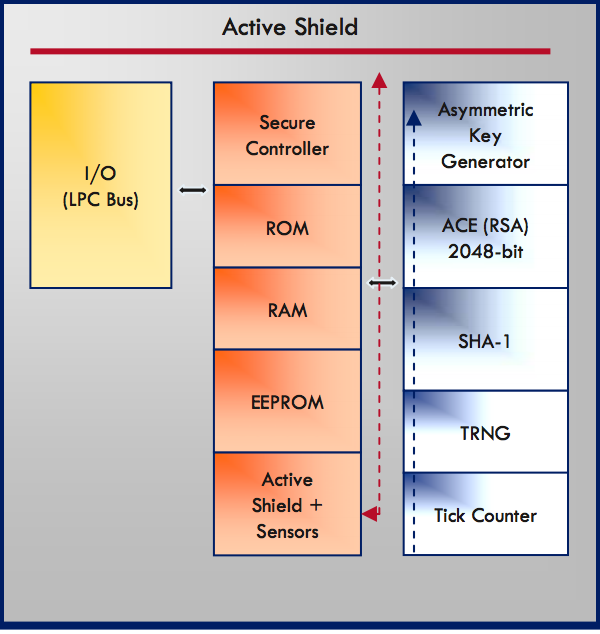
\includegraphics[width=1.0\linewidth]{tpm_hw.png}
\end{subfigure}
\begin{subfigure}{.40\textwidth}
  \centering
  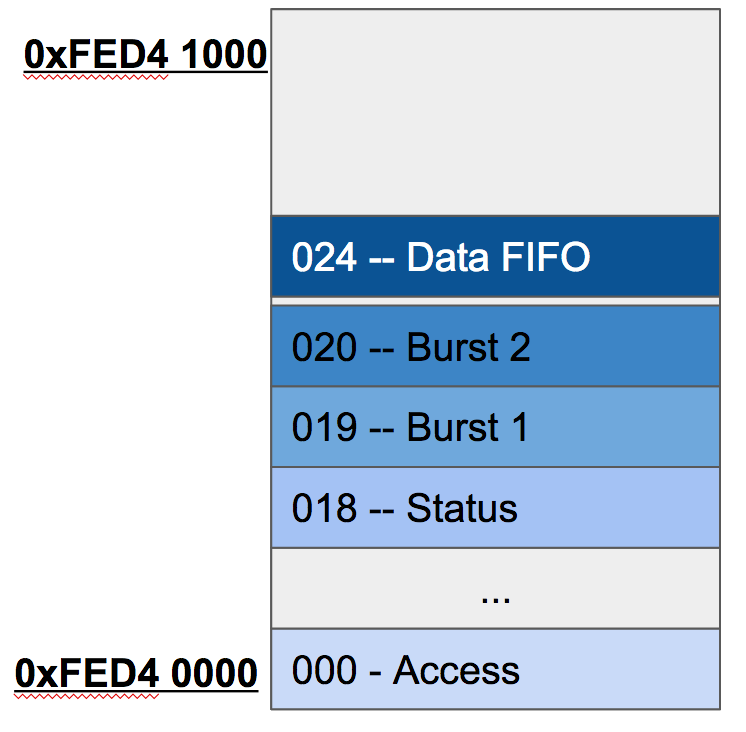
\includegraphics[width=1.0\linewidth]{tpm_regs.png}
\end{subfigure}
\caption{On the left we can see the registers of the TPM that are accessed by the CPU~. On the right we can see a HW block diagram of the TPM itself\cite{tpm-slides}.}
\label{fig:tpm_hw}
\end{figure}


\subsubsection{TPM Interface}

The CPU communicates to the TPM by reading and writing specific memory addresses.
These addresses allow the CPU to send multi-byte commands to the TPM and receive multi-byte responses, even though a single byte is read or written at a time.
The addresses and names of the registers can be seen in Figure~\ref{tpm_hw}.
I describe the registers below.

\begin{itemize}
    \item \code{Status} --- This register allows the CPU to know what state the TPM is currently in. Specifically, there are bits for  if the TPM is currently accepting or sending a command, or if the TPM is busy. Specific values can be written to this register to tell the TPM to start accepting a command, or to run a command that has been sent.
    \item \code{Burst} --- Reading this register lets the CPU know how many bytes can be read (if sending a command) or written (if receiving a command) at a single time.
    \item \code{Data} --- Reading this register reads one byte of data from the TPM~. Writing this register sends one byte of data to the TPM~.
\end{itemize}

% TODO: Should this be itemized or put into a graphic?
Sending a command serially to the TPM works in the following way.
First, the \code{Command\_Start} value is written to \code{Status}.
Second, the \code{Burst} register is read to see how many bytes the TPM can accept.
Next, the Data register is written to up to \code{Burst} times, until the command has been sent.
If the command is longer then \code{Burst} amount, \code{Burst} can be polled again until it becomes non-zero.
Finally, the \code{Command\_Go} value is written to \code{Status} and \code{Status} is polled until the TPM says that it has finished processing the command.

Receiving a command follows the process above, except that \code{Data} is read instead of written to.
Now that it is understood how commands are passed to and from the TPM, we can discuss the commands used by Google's Vboot.

\subsubsection{Platform Configuration Registers}

\begin{figure}
  \centering
  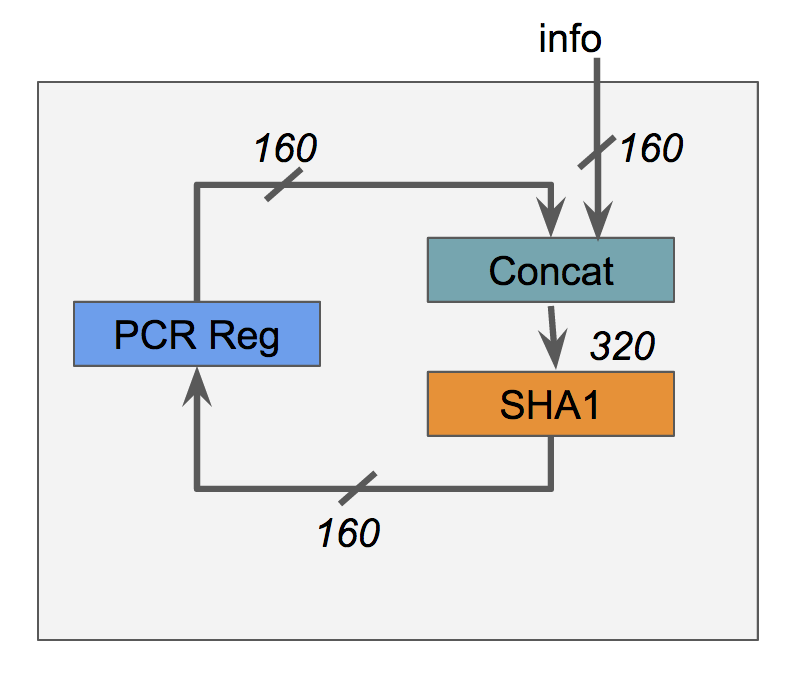
\includegraphics[width=0.4\linewidth]{pcr_alg.png}
  \caption{PCR extend Hardware Diagram}
  \label{fig:pcr_alg}
\end{figure}

One component of the TPM is called Platform Configuration Register, or PCR.
The goal of a PCR is to store measurements of the system state in a secure way. 
PCRs are secure storage because they cannot be written to directly, they are either extended or reset. 
PCRs are extended by concatenating the current the current PCR value with the input, and then storing the SHA1 hash of the result. 
Resetting the PCR changes the value to all zeros, although the PCRs used by VBoot have the reset functionality disabled.
There are three commands that deal with PCRs: \code{PCR\_Extend},
\code{PCR\_Read}, and \code{PCR\_Reset}.
PCRs can also be locked, meaning that they are then unable to be extended or reset for the remainder of the system's power cycle.
The TCG specifications of these commands are included in the Appendix.


The hardware diagram of PCR\_Extend can be seen in Figure~\ref{fig:pcr_alg}.
Because the PCRs store a SHA1 Hash, they are useful for taking the measurement of a system.  
Hashing is a one way cryptographic function that is used to protect the integrity of a message.
We can think of a hash as the fingerprint of a message, because it takes an arbitrary length of data and outputs a fixed length (20 bytes).
The PCRs are iteratively extended with measurements of the system, for example, the hash of the Read Only Firmware, then the hash of the Read Write Firmware, and then the hash of the Kernel.
The final result will be identical each time if and only if there were no changes in each of the things being measured.
By the definition of hashing, it is difficult also to find a fake configuration of the system that will hash to the same value as a correct configuration, meaning that if the hashes are equal it is reasonable to assume that the system is unchanged. 

Under specification 1.2, a TPM is required to have 21 PCRS, each PCR is 20 bytes
long and they are stored in the TPM's non-volatile storage.
Each power cycle the PCRs are reset to all 0's.

\subsubsection{Secure Storage}

% TODO: Talk about the NV Storage Commands

\subsection{SHA}

\subsection{QEMU Emulation}\label{qemu_em}

\begin{figure}
  \centering
  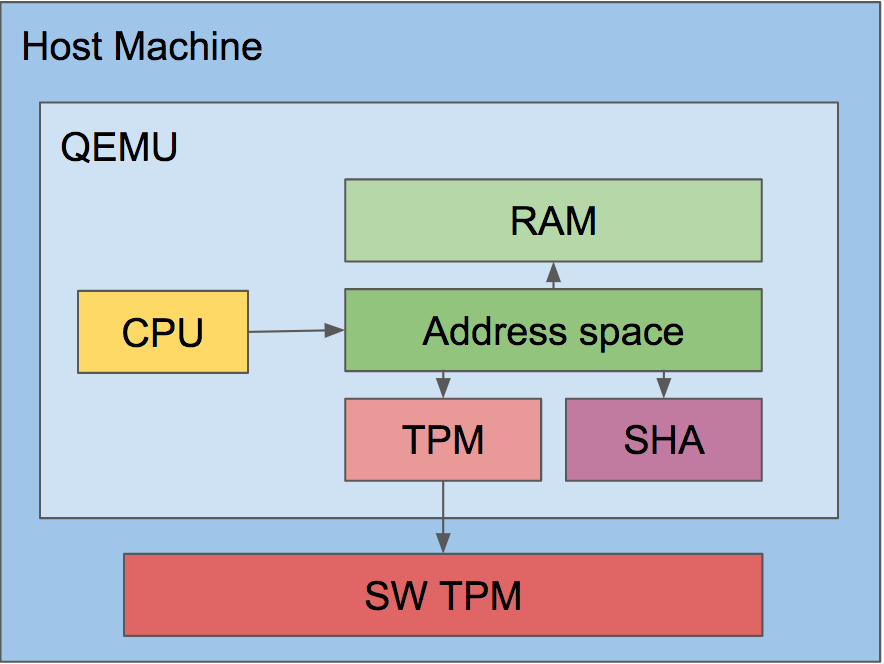
\includegraphics[width=0.4\linewidth]{qemu_layout.png}
  \caption{The QEMU layout. We can see here how the CPU and other hardware modules write RAM, and how some QEMU modules are interfaces to external software libraries.}
  \label{fig:qemu_layout}
\end{figure}

QEMU~\cite{qemu-site} is an open source emulator that is used in the report to emulate the computer running Vboot.
For this project it is used to emulate a 32 bit i386 CPU with a Memory Mapped TPM and SHA module.
To run code, I am relying on QEMU's ability to boot any image that starts with a defined multi-boot header~\cite{multiboot}.
QEMU then supplies its own bootloader, which is responsible for initializing RAM, putting the processor in 32 bit mode, and loading the image off of disk.
As we will see in Section~\ref{coreboot}, for Chromebook this job is normally taken care of by Coreboot, but for the purposes of this report it was easier to use QEMU's built-in bootloader.

The QEMU code (included in the appendix and the github link), was based off of a project developed for Open Source at Princeton by me and Lance Goodridge.
The Open Source project allowed students to build their own Operating System from scratch and develop it within QEMU\@.
The Open Source project was repurposed by this thesis for its well-organized Makefile, linker script, and multi-boot header.
These tools allowed me to create and compile a standalone C file that could hook into the Vboot repository and run Google's Verified Boot within QEMU's virtualized Hardware.

The QEMU emulator was modified to add a TPM and a SHA module, but as mentioned in Section~\ref{flash_mem} it does not include the Flash Memory.
While the Flash Memory is important as a Root of Trust in the System, its purpose is very simple.
Its main function is to provide read-only storage, and this is not a property that is difficult to be checked.
Instead of adding Flash Memory to the QEMU emulation, I load the Vboot code in with the image using the linker script. %TODO link to Linker script
The linker script loads in different sections that would correspond to the Flash Memory, and these sections are accessed normally in RAM instead.

% TODO: Get the SHA working
% Using my own SHA implementation, close to the one used by coreboot

\subsection{Instruction Level Abstraction (ILA)}

I am using a tool to create an Instruction Level Abstraction (ILA) of Hardware.
The ILA is used to create an abstraction of the TPM and SHA module that can be
easily verified.
Verifying Firmware is difficult because it accesses Hardware by writing to
memory-mapped registers that trigger Hardware events.
Using a Software only model checker like CBMC will only see these writes
and reads to addresses, and it will not understand that a single write
corresponds to an entire Hardware operation.

ILA provides a way to ``precisely capture updates to all firmware-accessible
states spanning cores, accelerators, and peripherals''\cite{ila-template}.
An ILA is created from either a C or Verilog program that represents the
Hardware.
This program is referred to as the Oracle, and the resulting abstraction from
the ILA will capture the Oracle's behavior. %TODO: bad wording
A programmer must manually create an ILA template that describes each state of
the Hardware and each of the states possible updates.
The template is focused on the ``instructions'' of a Hardware module, and it is
programmed using the standard Fetch, Decode, Execute module of a Computer CPU\@. 
Completing the template involves manually specifying hardware state, possible
inputs (Decode), and possible updates (Execute).
Once the template is complete, the ILA library uses the Oracle to fill in the
holes of which Decode values correspond to which functions the system Executes.

The ILA template that is created captures the interface of the Hardware.
It produces an abstraction that is aware of how the Hardware reacts to Reads and
Writes of specific Registers.
This template can be connected back with the Firmware such that verification can
happen across the Firmware-Hardware boundary.

\end{document}

\documentclass[../report.tex]{subfiles}
 
\begin{document}
\onehalfspacing

\newpage
\section{Software Design}

% It is important for security reasons that Vboot itself is unmodified and cannot be removed by a hacker wishing to replace the system's firmware or OS undetected.
% For this reason the Vboot code is stored and executed out of the Read Only Section of Flash which is designed to be unmodifiable without tampering with the system's hardware.

This section will discuss the Software and Firmware implementation of Verified
Boot. 
Verified Boot (Vboot) is a secure boot implementation only runs code that has
been signed by Google and is untampered.
Images that have been recognized as security risks will not be loaded and the system will restart into a Recovery Mode.
Google has implemented different modes that Vboot can boot with and these modes alter the program flow and security guarantees.
In this section I will discuss the security promises made by the system as well
as the attack vectors that are not considered.
I will also discuss relevant data structures and program flow.

\subsection{Security Promises}

The main purpose of Chrome OS's verified boot is to provide relative security to the end user without sacrificing usability or functionality. 
In its mission statement, verified boot is designed against an ``opportunistic hacker''~\cite{vboot-design-doc}.
Vboot protects against vectors of attack that are relatively quick to exploit.
Vboot will realize any attack or modification on the next boot cycle.
Once an attack is realized Vboot will get the system back to a secure state.
An example of an attack that would be caught by Vboot would be the installation
of a malicious kernel driver to act as a keylogger, or the replacement of the
current kernel with an older version that has known vulnerabilities.

There are many attacks that Vboot is not able to recognize or protect against.
For example, Vboot does not make any promises to the safety of the system once the kernel is running and the user has control. 
Any attacks that are outside of the kernel (in userspace) would remain
undetected because they would not modify the kernel.
For example, changing the Web browser to use a proxy that collects information
would not be considered a kernel attack.
Userspace programs by definition have less access to the system and this reduces the severity and influence of the attack.
Possibly one of the biggest flaws is that any attack to the kernel during
runtime would remain until the system was powered down.
In certain situations could provide plenty of time for an attack to steal valuable data.
However, such an attack is outside the scope of this paper.

\subsection{Verified Boot Flow}

In order to divide the code modularly and have Verified Boot be extensible for current and future platforms, Google has split the process into three main sections as seen in Figure~\ref{fig:vboot_stages_overview}.
This also allows Google to make the Read-Only stage as small as possible, which is good because bugs in this stage cannot be fixed.
These sections are referred to as Read-Only (RO) Firmware, Read-Write
(RW) Firmware, and Kernel.
These sections are run in sequence with each section verifying the section that comes later.
In this way the root of trust starts from the Read-Only portion and builds until the system has booted completely.
For the scope of this document we will discuss only the Verified Boot process for the verification between RO Firmware and RW Firmware. 
This verification contains more interesting control flow, and process is essentially repeated for the verification between the RW Firmware and the Kernel.

\begin{figure}
\begin{subfigure}{.4\textwidth}
  \centering
  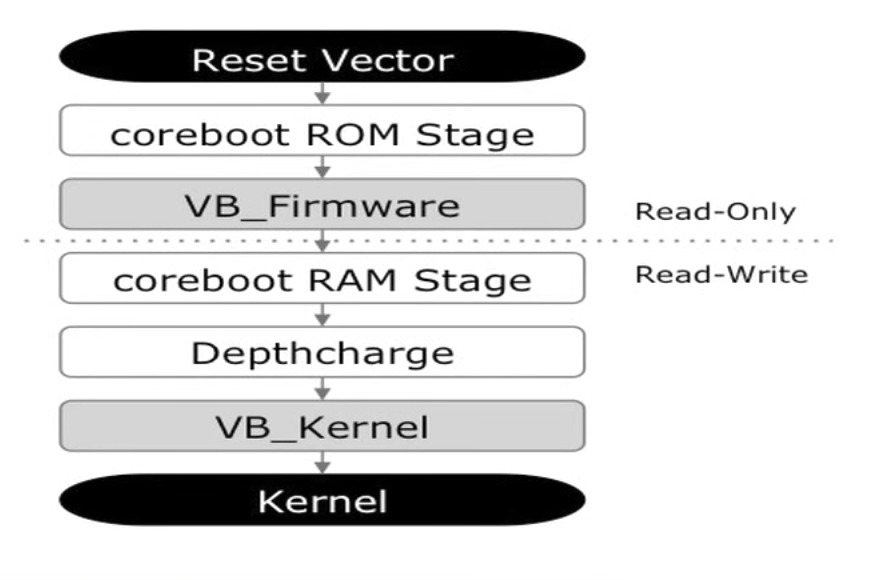
\includegraphics[width=1.0\linewidth]{vboot_stages_overview.png}
\end{subfigure}
\begin{subfigure}{.60\textwidth}
  \centering
  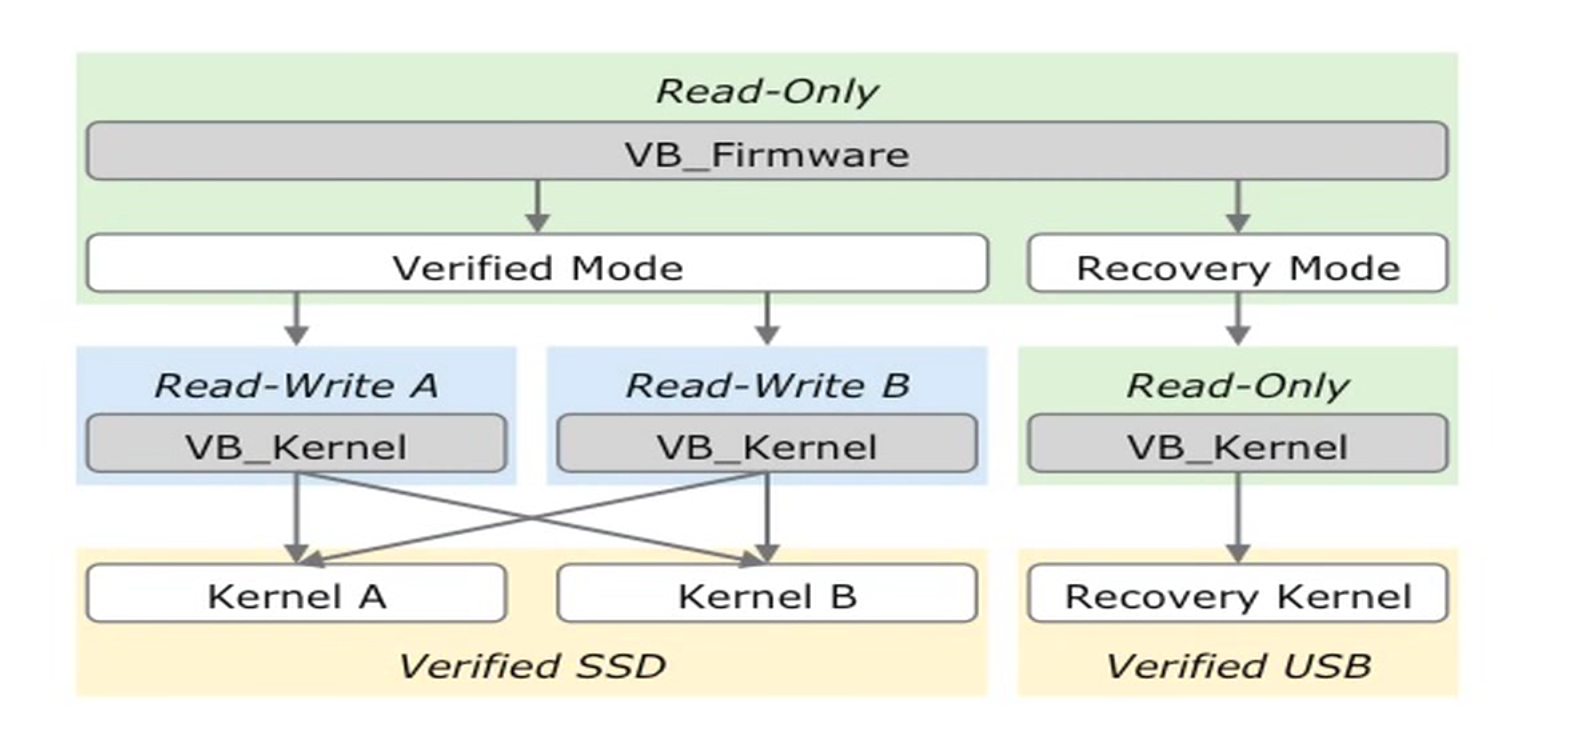
\includegraphics[width=1.0\linewidth]{vboot_stages_AB_recovery.png}
\end{subfigure}
\caption{The left image shows the stages of Vboot Firmware. The right image
shows the different boot paths, and data locations. Both make the distinction
between Read-Only and Read-Write memory.}
\label{fig:vboot_stages_overview}
\end{figure}

The RO Firmware runs first and as such is the root of trust for the entire platform.
It is responsible for verifying the RW Firmware image and it contains all of the code and hardware drivers it needs to accomplish this task.
It verifies the RW Firmware Image signature using Google's main public key.
This public key is packaged with the RO Firmware and is also read only so it is guaranteed to be secure.
The RO Firmware is also responsible for handing the main control of Vboot, and this includes the transitions between Developer Mode, Safe Mode, and Recovery Mode.
These transitions will be described in more detail in Section~\ref{sec:boot-modes}.

\begin{figure}
  \centering
  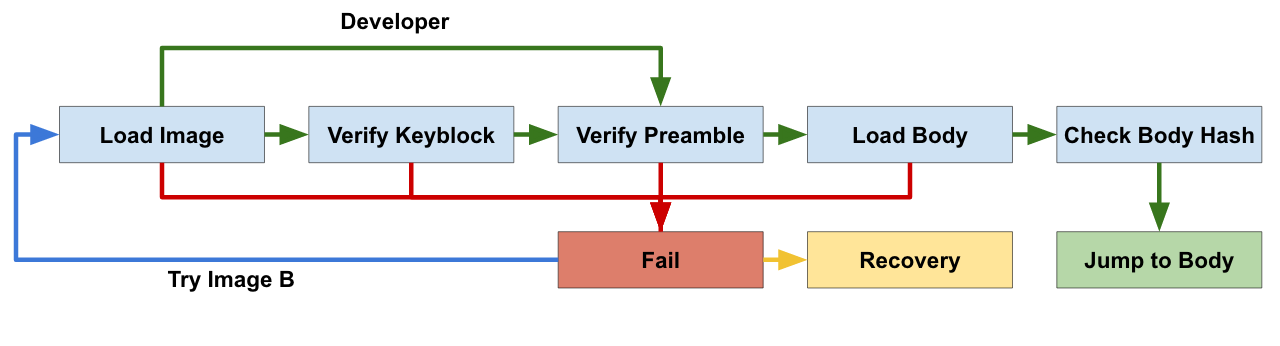
\includegraphics[width=0.8\linewidth]{verification_flow.png}
  \caption{The logical flow for verifying the firmware image. Notice
  the different path for Developer mode, and the possibilities for
  failure.}\label{fig:verif_flow}
\end{figure}

The stages that the RO Firmware goes through include loading the image, verifying the keyblock, verifying the preamble, loading the body, verifying the body, and then executing the code in the body. 
These stages can be seen in Figure~\ref{fig:verif_flow}.

Loading the image consists of copying the image out of the Flash Memory (Section~\ref{flash_mem}) and into RAM where pointers to the image are passed around on the C call stack.
Verifying the Keyblock consists of using its signature, which is a hash of its full information that is signed by Google's Private key.
Google's Public Key, which is stored in Read-Only Memory, is used to decrypted the signature, so that it is now only a hash of the Keyblock.
Finally, the entire Keyblock is hashed, and the two are compared.
If the hashes are not equal, then the Keyblock currently viewed by the machine is not the one that was originally signed by Google.

The Preamble is verified in the same way, except that a different Private and Public Key pair is used.
The Keyblock holds the key that is used for the Preamble's signature.
The Keyblock is used so that Google has the ability to change the encryption
type of the Preamble and Firmware if they wish.
Google's Main Public Key is stored in Read-Only memory, so it cannot be changed.
This hierarchy of keys also allows Google to be less careful with their ``lower
security'' keys because they can change them via update if the key is
compromised.

After the Preamble is verified, the Firmware Image is hashed and compared
against the hash stored in the preamble. 
The hash in the preamble has already been verified because the preamble was
signed, so this verifies that the Image is correct and unmodified. Finally, the
system jumps to the Image and begins to execute the code for the main Firmware
and Operating System.


\subsection{Boot Modes}\label{sec:boot-modes}

Vboot has three major boot states that influence the program's behavior.
The first state is the Secure state which goes through the full process of Verified Boot normally.
The second state is the Recovery state which allows for a broken machine to
format all memory and revert to a secure state.
The third state is the Developer state and in this state the RSA signature is not verified.
The Developer state exists so that hobbyists can write their own firmware boot code and run operating systems other than Chrome OS\@.

The transitions allowed between the states can be seen in
Figure~\ref{fig:mode_fsm}.
On each transition, Vboot is responsible for taking steps to ensure that
security is preserved. 
These responsibilities are also seen in the figure.

\begin{figure}
  \centering
  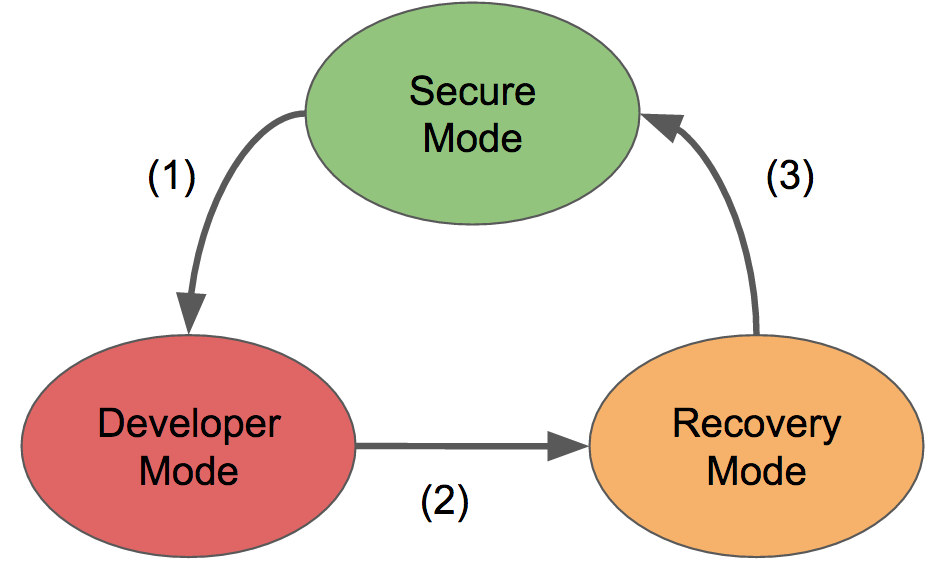
\includegraphics[width=0.4\linewidth]{mode_fsm.png}
  \caption{The FSM for the boot modes. \\
  1. The TPM's nonvolatile storage and keys are wiped. The user's data
  is erased. \\
  2. The laptop is booted into Recovery, Vboot installs a Chrome USB.
  \\
  3. The TPM's storage goes through reconfiguration. The entire disk is wiped.
  \\}\label{fig:mode_fsm}
\end{figure}

\subsubsection{Developer Mode}

Developer mode poses interesting security questions to Verified boot because it essentially disables the security guarantees and allows the system to move into an insecure state~\cite{developer-mode}. 
There are various security requirements around the Developer state transition.
First, a physical presence is required to fully complete the developer mode transition. 
This means that a person must sit at the computer once it has been rebooted and press a certain key combination (Control + D) when the developer mode screen appears.
The physical presence exists such that developer mode cannot be enabled through an off-site software attack without the user's knowledge.
The developer mode screen is referred to internally as the ``Scary Screen'', and its purpose is also to prevent users from being tricked into enabling developer mode by an external phishing party.
Once Developer Mode is enabled, the system can no longer claim guarantees about the boot process or its own secure storage.
In order to prevent an attacker from enabling Developer Mode so that they could read secure storage, Vboot wipes all secure storage on the transition into Developer Mode.
The secure storage that is wiped includes the RSA keys and various secrets stored in the TPM and the partion on disk where user data is stored.
Wiping this data on the transition is necessary to the confidentiality of the system and failure to do so is a security risk.

These precautions are also taken on the transition from Developer Mode to Safe Mode. 
If secure storage is left untouched moving from Developer Mode to Safe Mode, then an attacker would be able to place potentially malicious information in secure storage.
The assumptions that Google places on secure storage require that it can only be written to and read from by Google.
The platform will not be able to recognize if secure storage is in an insecure or malicious state and so wiping it is the easiest way to ensure that the platform has full control.
On the transition from Developer to Safe Mode, the system has to go through Recovery Mode.

\subsubsection{Recovery Mode}

Recovery Mode is responsible for getting the system back to a secure state.
Recovery Mode will be activated automatically when an error is recognized in Vboot.
This error could range from hardware failures to a corrupted image to a detected attack on the system.
When the system boots into Recovery it is for a Recovery Image stored on external memory, either on an SD card or a USB drive.
The path for recovery uses a different RSA key for modularity and this recovery key is also stored in Read Only Flash in order to be unmodifiable.
Once the recovery image is verified to be secure and unmodified, the image is loaded off of the external storage and it is used to replace the images currently stored on the device.
Recovery mode is also responsible for wiping secure memory, including the user's disk partition and TPM's secure storage.
If Recovery completes successfully, the system is in a secure state and Vboot can then continue safely.
From a user perspective, Recovery is an easy way to wipe the device and restore it to Factory Settings.
Recovery is also the only way to roll the device back to an early image, and this rollback is sometimes necessary if there are known problems with a newly uploaded image.

\subsection{Data Structures}\label{sec:data-structures}

To start understanding the Vboot verification process, it is necessary to talk about the data structures that are used throughout. 
These data structures are populated by the Firmware Image that is being
verified. 
Through this section I will start at the highest hierarchical level of data structure then explain the structures that are contained within.

\subsubsection{Firmware/Kernel Image}

\begin{figure}
    \centering
    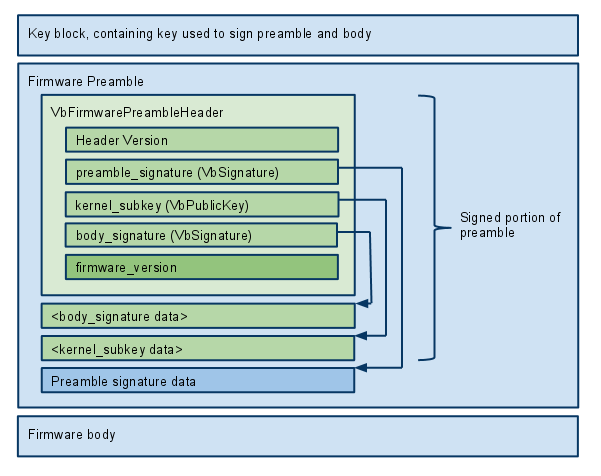
\includegraphics[width=0.6\linewidth]{fw_image.png}
    \caption{Layout of the Firmware Images~\cite{vboot-data-structures}}
    \label{fig:vboot_images}
\end{figure}

The actual image is not a data structure but a chunk of data that is stored contiguously in non-volatile memory.
The image structure, as seen in Figure~\ref{fig:vboot_images}, consists of three parts: a key block, a preamble, and the main body of the image.
The key block is verified first, and it is verified by the main RSA key stored in Read Only memory.
Once the key block has been shown to be safe, the RSA key located within will be used to verify the preamble.
The preamble contains the hash of the image's body.
The image's body contains the code that is going to be run next and it is checked against the hash stored in the preamble.
The preamble also contains the RSA key used to verify the key block of the Kernel image.

\subsubsection{Key Blocks}\label{sec:key_block}

\begin{figure}
\begin{subfigure}{.5\textwidth}
  \centering
  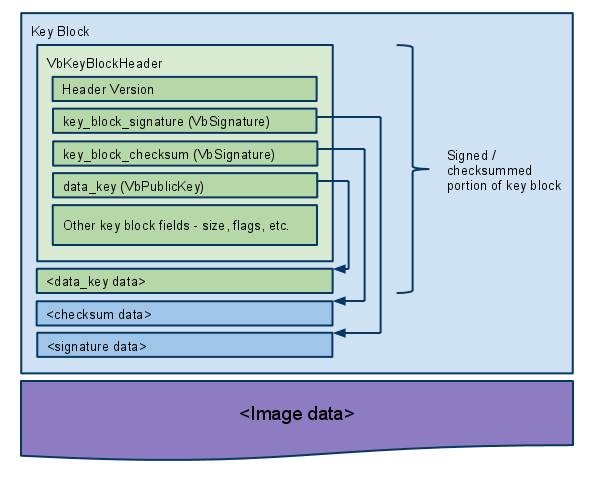
\includegraphics[width=1.0\linewidth]{vboot_keyblock.png}
\end{subfigure}
\begin{subfigure}{.20\textwidth}
  \centering
  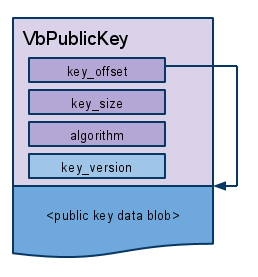
\includegraphics[width=1.0\linewidth]{vbpublickey.png}
\end{subfigure}
\begin{subfigure}{.20\textwidth}
  \centering
  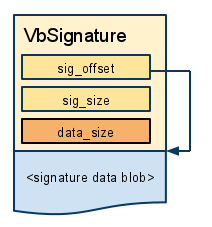
\includegraphics[width=1.0\linewidth]{vbsignature.png}
\end{subfigure}
\caption{The Keyblock data structure and Metadata for Keys and Signatures}
\label{fig:vboot_keyblock}
\end{figure}

The Key block is the first part of the image that is validated and it is used to validate the rest of the image.
The Key block is the data structure that allows a hierarchy of RSA keys to be used during Vboot.
Figure~\ref{fig:vboot_keyblock} shows the structure of the keyblock. 
The key block flags that are mentioned are used to determine which mode of Vboot the Keyblock is valid in. 
There are 4 possible boot modes corresponding to the combination of the two binary options, Developer and Recovery.
% info located in vboot_struct.h

Within the keyblock there exists data structures for a public key and a signature.
Google has added the ability to change their encryption strength.
They have added support for RSA 1024, 2048, 4096, 8192 and for SHA 1, 256, 512, for a total of 12 different possible algorithm combinations.

\subsubsection{Google Binary Block}

% info found in gbb_header.h
The Google Binary Block (GBB) is a part of Vboot's Root of Trust.
It is a data structure stored in Read-Only memory that is initialized and configured in the factory at the laptop's creation.
It contains the Root and Recovery RSA keys, a host of flags that affect boot operation, and the bitmaps used for various boot screens.


\subsection{Code Organization}

Like most modern operating systems, Chrome OS is written in C.
Like Linux, Chrome OS is maintained using Git for version control. 
Git is a diff-based, non-centralized version control system that makes it easy for programmers to share code, rollback changes, and maintain separate branches of the same codebase~\cite{git}.
Google has built a tool called ``repo'' that is used on top of git~\cite{repo}. 
Repo is a tool to manipulate multiple code repositories. 
It's primary benefit is that it allows a company to specify how multiple git repositories should be installed and placed within a given file-system.
This is both helpful and necessary as Chrome OS consists of over one thousand different external and internal repositories. 

Coreboot, vboot\_reference, depthcharge, are the repositories used for the firmware boot process.
The flow of Verfied Boot through the repos can be seen in
Figure~\ref{fig:code_repos} and the purpose of each repo is described below.

\begin{figure}
  \centering
  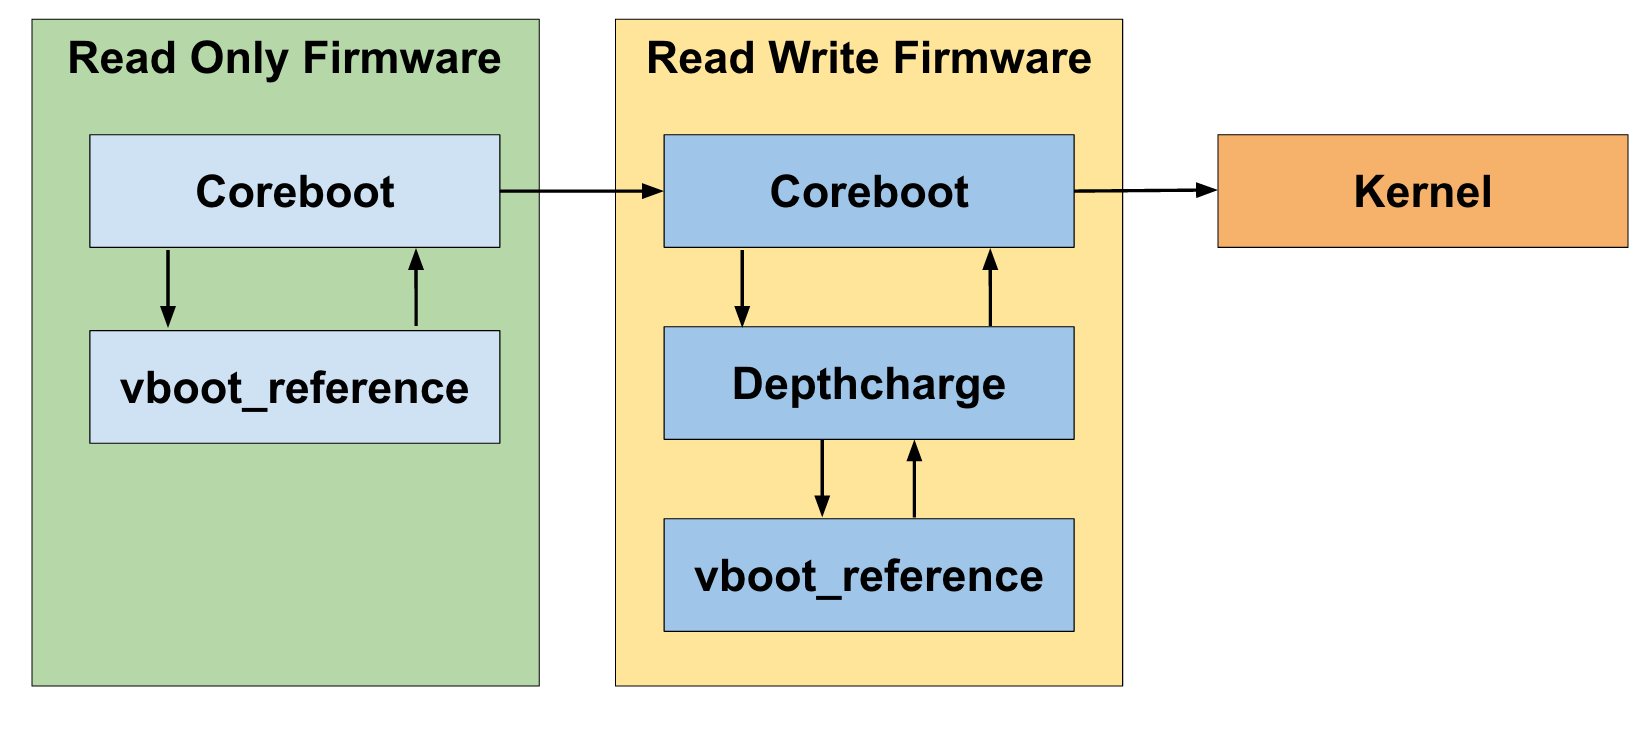
\includegraphics[width=0.8\linewidth]{code_repos}
  \caption{ChromeOS's boot flow goes through Coreboot, Depthcharge, and the Vboot Library twice for Firmware and Kernel verification}\label{fig:code_repos}
\end{figure}
\begin{figure}
  \centering
  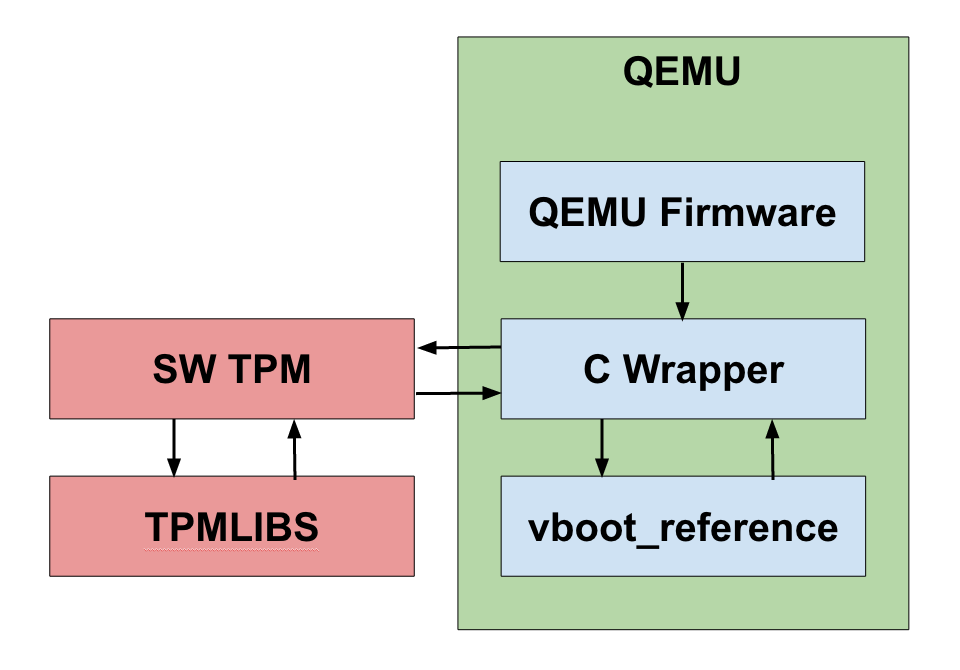
\includegraphics[width=0.45\linewidth]{qemu_repos}
  \caption{This report's boot flow uses QEMU's default bootloader Firmware, then
  a created C wrapper for the TPM and Debugging Output, and Vboot for the
  verification}
\end{figure}

\subsubsection{Coreboot}\label{coreboot}

Coreboot is a fully Open-Sourced alternative to traditional BIOS implementations.~\cite{coreboot}
It is lightweight and is configured to implement the full standard of the Unified Extensible Firmware Interface (UEFI).
Google has chosen Coreboot because of its small code footprint, full extensibility, and the fact that it is available freely as an Open Source project.

The Coreboot code is responsible for doing very early initialization code on the main CPU\@. 
% This includes things like setting up the GPIO pins, enabling hardware interrupts, setting up a large stack in RAM, and providing driver callbacks to the payload that it will eventually call.
Coreboot is setup so that once a baseline level of initialization is complete, it passes control to another section of code called a ``payload''~\cite{coreboot-payload}.
This payload is responsible for initializing the more specialized drivers, and the concept of a payload means that Google can keep support more hardware without altering the Coreboot source code.
The payload that Coreboot calls to further initialize the Chromebook is Depthcharge.
% Init done in src/mainboard/google/{link}/romstage.c

% \subsubsection{DepthCharge}
% 
% Depthcharge contains the minimum number of drivers necessary for the virtual boot to work successfully~\cite{depthcharge-codebase}. 
% The important drivers include the TPM, I2C, the EC, SPI and SPI Flash, and the display~\cite{depthcharge-slides}.
% Once the drivers are initialized successfully, Depthcharge creates the necessary structures for Vboot and then passes control into the Vboot library.
% 
% Depthcharge is Google's repo that holds platform dependent code.
% The different branches in the repository hold different drivers as they are needed for each of the Chromebook's hardware.

\subsubsection{Vboot\_reference}

The vboot\_reference repo contains all of the control and algorithms for the vboot process~\cite{vboot-codebase}.
The repo is designed such that it does not rely on any knowledge about the platform.
If a function requires usage of a driver or something that is board specific, it will make a callback into Depthcharge which will provide the relevant information.

One of the more helpful features of the vboot\_reference repo is that it can be
built in a stand-alone fashion as a C archive file.
More information about building the project can be found in the appendix, but
this feature allowed the Vboot functions to be placed into the QEMU environment
easily, and it can be adapted for many different types of hardware.

\subsubsection{Software TPM}

This project uses a software-emulated TPM instead of a physical chip. 
This emulated TPM implements all of the TPM's functionality as defined by the
TCG Standards.
The fact that the emulation was software allowed the TPM to be put into various
states easily without requiring a physical reboot of the system.
Once the emulated TPM was passed to QEMU, it was accessed through the same
Memory Mapped Registers as the Hardware TPM outlined in Section~\ref{sec:TPM}.
This was very helpful because it meant that the Vboot TPM functions would work
with the emulated TPM.

The Software TPM was taken from a series of repositories created by IBM's
Stefan Berger. 
These repositories emulated the TPM functions\cite{TPMLibs}, the TPM Command
Fifo\cite{SWTPM}, and the TPM Register Interface\cite{TPMQEMU}. 
More information about installing the Software TPM libraries can be found in the
appendix.

% TODO: C Wrapper Sub section


\end{document}

\documentclass[../report.tex]{subfiles}
\def\code#1{\texttt{#1}}
\begin{document}
\onehalfspacing

\pagebreak
\section{Verification}\label{sec:Verif}

In this section I will discuss the security properties used by each section of
Verified Boot. These properties have been mentioned earlier, but they are
formalized in this section.
Later in the section I verify these properties on the Hardware and
Software system that I outlined in Section 2 and Section 3.
Properties in software are checked using CBMC, where properties across the Hardware-Firmware boundary are checked using ILA.

All properties are being defined on the Read-Only Firmware of Verified boot.
The code for Verified Boot is taken from an unmodified vboot\_reference repository provided by Google. 
When secure promises cross the Hardware-Firmware boundary, they are evaluated
using the Hardware I selected in Section 2.
The Firmware that interacts with this Hardware was created by me, however it was 
modeled after the Firmware originally found in Google's Coreboot repository. 
If Google released the sources for their Hardware, then this testing could be
performed with no modification to the source code. 

%\subsection{Read-Only Fw Purpose}
%The Read-Only Firmware's purpose is to provide an initial configuration of the board's hardware and to verify the block of code that has been provided as the Read-Write Firmware.
%The RO Firmware requires the SHA and RSA accelerators to do cryptographic functions, and the TPM and Flash for secure storage.
%If Developer Mode or Recovery Mode are enabled then the Keyboard driver is required for user input and the Display driver is required for updating the user with the boot status.
%If Recovery Mode is enabled then the USB and SD drivers are required so that the recovery image can be read off of external storage.
%Implementations of all of these drivers are packaged with the RO Firmware so that the Vboot library can succeed.
%
%The first thing that RO Firmware is responsible for is loading in all of the Flash memory to RAM so that it is more easily accessible. 
%After Flash memory is in RAM, data structures like the GBB and the Firmware Image are populated by reading the flash map, which is always stored at a set location (see Figure~\ref{fig:fmap}).
%Once the data structures are populated and the hardware drivers are loaded, the RO Firmware moves into the Vboot library to verify the firmware image.
%
%% RO FW destinations
%The RO Vboot is responsible for checking the validity of the firmware image validity and either executing the code within the firmware image or failing appropriately.
%If the firmware image is insecure or the verification process fails for other reasons, it is likely that the system will be rebooted into recovery mode. 
%RO Vboot is responsible for setting a 32 bit flag known as a ``recovery reason'' for failure. This reason influences the Recovery process and is stored in the read write portion of Flash so that it is consistent across boots. 


\subsection{RO Firmware Properties}

The properties that we will be checking can be separated into 4 categories: array accesses, program flow, hyperproperties, and correctness.
The array access property restricts the writeable addresses in memory to valid array boundaries. 
Program flow properties refer to the execution path and function call stack throughout the program.
Correctness properties refer to facts about the code such that, if things were
designed successfully, certain states should not be reached.
Together these categories of properties should encompass each of claims that the system makes about security.

These properties will be specified in Computation Tree Logic (CTL). 
CTL adds temporal distinctions over propositional logic and this allows one to easily describe how a system changes over time.
The boolean connectives in propositional logic are $\lnot$ for NOT, $\land$ for
AND, $\lor$ for OR, and $p \to q$ for $p$ implies $q$.
CTL describes how propositional logic changes through time.
In CTL $Xp$ indicates that $p$ is true in the next state; $Fp$ indicates that $p$ is true eventually; $Gp$ indicates that $p$ is always true.

\subsubsection{Memory Access Locations}

Memory accesses in C are very important because the language allows for arbitrary addresses to be accessed. 
Addressing arrays before their starting address or after their final address is known as a buffer overrun and it is one of the most common security vulnerabilities. 
Buffer overruns allow a program to write or read to arbitrary memory. 
In this program, a buffer overrun could be used to modify the RSA public keys after they have been read in from secure storage, or it could modify the firmware image after it has been verified as secure. 
Such modifications would defeat the security purposes of Vboot and for this reason it is important to prevent the accessing of arrays past the array boundaries.
We can represent correct array accesses through formal specification using the formula below.

\begin{equation}
    G(a \to (i > 0 \land i < size(ptr)))
\end{equation}

In this equation $a$ is any array access, $ptr$ is the start of the array and $i$ is the access offset.
This equation states that for every memory access, the index is greater than 0 so it cannot access memory before the array,  and the index is smaller than the size of the array so memory after the array cannot be accessed.
Luckily, this problem is common enough that CBMC provides checking by default.
However, This equation on its own is not strong enough to provide array access security for verified boot. 
This is because Vboot uses pointer manipulation throughout in order to access structures and data within the Firmware Image. 
Verified boot reads the image in as one contiguous blob and then uses size and offset variables to read more information.
CBMC is not able to detect that this pointer manipulation is an out of bounds array access so this must be manually checked through the use of assertions each time something within the image is accessed.
The pointer manipulation can be expressed formally through the following formula.

\begin{equation}
    G(s \to \text{offset}(\text{struct}) + \text{size}(\text{struct}) <
    \text{size}(\text{img}) \land \text{offset}(\text{struct}) > 0)
\end{equation}

In this equation $s$ is each time a structure is created from a pointer dereference, $struct$ is the structure, and $img$ is the image that it is being pointed to.
The equation states that the offset and size of the struct do not go past the edge of the image and that the offset of the struct does is not negative or before the beginning of the image.

Together these properties state that array accesses must be in bounds and that structure dereferencing must be in bounds of the image that is being referenced.
As these are the two memory referencing techniques that have the potential for overrun, these properties protect the system against overrun attacks.

\subsubsection{Program Flow properties}

There needs to be an ordered constraint on the flow of the program. 
If the program flow is described formally then it will be easy to check that all stages of secure boot were called and in the correct order.
This will catch incorrect programs that skip steps and therefore skip verifying the image, or programs that execute steps out of order and therefore access data that has not been verified yet.
The graph for program flow is shown in Figure~\ref{fig:verif_flow}.
When verifying the flow of Vboot it is necessary to note that there are two firmware images stored in the system, Image A and Image B, and either can be used in the Vboot process. 
It is also necessary to note that Developer mode will skip a step in the verification process, and that this skipped step is a valid part of the Vboot flow.

Let $s_i$ correspond to the ith stage from Figure~\ref{fig:verif_flow} and $s_{ai}$ or $s_{bi}$ correspond to that stage for Image A or Image B respectively.

The equation below states that at any time, we must be in at least one of five stages for either image A or image B.
% Must be in a defined state
\begin{equation}
    G(\bigvee\limits_{i = 0}^{4} s_{ai} \lor s_{bi})
\end{equation}

The equation below states the transitions available for Image A.
Each i\textsuperscript{th} stage can transition either to itself or the following stage.
Image A also has the ability to fail and have a transition immediately to the first stage of verifying Image B.

% Image A transitions to next or to B
\begin{equation}
    G(s_{ai} \to s_{ai} \lor s_{ai+1} \lor s_{b0})
\end{equation}

Now we will describe the state transitions for Image B. 
They are similar to Image A but Image B is always tried secondarily and can only transition to the next stage. 
Image B cannot transition back to verifying Image A or there would be the possibilities of an infinite loop of verifying incorrect images.

% Image B transitions to next
\begin{equation}
    G(s_{bi} \to s_{bi} \lor s_{bi+1})
\end{equation}

The final equation refines the transition for state $s_0$ for Image A and B.
In Figure~\ref{fig:verif_flow} we can see that state $s_0$ can transition to either $s_1$ but it also has a special transition to $s_2$ that is only valid if Developer Mode is enabled.

% State 0 can skip state 1 if in Developer
\begin{equation}
    G(s_0 \to (s_0 \lor s_{1} \lor (M_D \land s_{2})))
\end{equation}

All together these equations fully describe the program flow graph in Figure~\ref{fig:verif_flow}. 
If these hold then steps will not be skipped in the verification process and we can be assured that verification of the image will be attempted in order.

% \subsubsection{Hyperproperties}

% TODO: Look at this later
% Verified boot contains many stages and each stage holds multiple flags and meta-data. 
% We want to make sure that untrusted information does not influence our booting sequence, be

\subsubsection{Correctness properties}

Correctness properties refer to the code itself and help to determine if it has been written correctly.
For Verified Boot, correctness properties are focusing on the correct attestation of the image and attempting to guarantee that an incorrect image cannot be marked as correct and loaded for execution.
For example, the following property states that if the system is not in developer mode and the signature verification fails, then the system will eventually reach the failure state for that image.
It is important that failure and passing is tracked on an image basis because it is possible for Image A to have a bad signature but for Vboot to verify and load a correct Image B.

% Signature is correct when not in Dev mode
\begin{equation} \label{eq:sig_cor}
 \lnot M_d \land \lnot \text{verifySignature(img, rootKey)} \to XF (\text{img.pass} = F)
\end{equation}

The following property states that if the hash of the image data does not match the hash stored in the image, then that specific image will eventually fail.

% Hash is correct always 
\begin{equation} \label{eq:hash_cor}
    \text{hash(img.data)} \neq \text{img.hash} \to XF (\text{img.pass} = F)
\end{equation}

The next property checks against the rollback attack. 
Rollback states that all image versions must be greater than or equal to the last seen image version that is kept in secure storage. 
This property claims that if the image version is lower than what is seen in secure storage, then the image will eventually fail.
Rollback is disabled on Recovery Mode and the property below reflects this fact.

% Version should be greater than previously seen when not in recovery
\begin{equation} \label{eq:rollback}
    \lnot M_r \land (\text{img.version} < \text{prevVersion}) \to XF (\text{img.pass} = F)
\end{equation}

The next property checks that if both images fail, then the Vboot process will fail and the system will eventually reboot into recovery mode.

% If both images fail then boot to recovery 
\begin{equation} \label{eq:both-fail}
    \lnot \text{imgA.pass} \land \lnot \text{imgB.pass} \to XF (\text{pass} = F)
\end{equation}

% TODO: maybe add a Dev wipe property

% TODO: maybe add a hardware return correctly property
% TODO: maybe add that if hash(image) = img.hash -> image = img

In the equations above, img refers to the image to be verified (either Image A or Image B)  and rootKey is Google's public key that has been loaded out of the gbb.
$M_d$ refers to developer mode being active and $M_r$ refers to recovery mode being active.
Img.version is the RW firmware version and prevVersion is the last seen version that is stored in the TPM\@.
These properties will be proved contrapositively, meaning that when verified boot passes we will check that the antecedent is also false.


\subsection{CBMC}

CBMC is a Bounded Model Checking program for the C language that is released by
Carnegie Mellon. 
A Bounded Model Checker is a tool that performs Formal Verification.
Model checking is a way to exhaustively prove whether a given model meets its
specification.
Model checking typically uses propositional logic or temporal logic. 
At its core, CBMC transforms a C program into binary logic and
then uses a SAT solver to check it against the user's specification. 
The specification is user defined, using an API of C functions defined by the
CBMC library. 

\begin{figure}
  \centering
  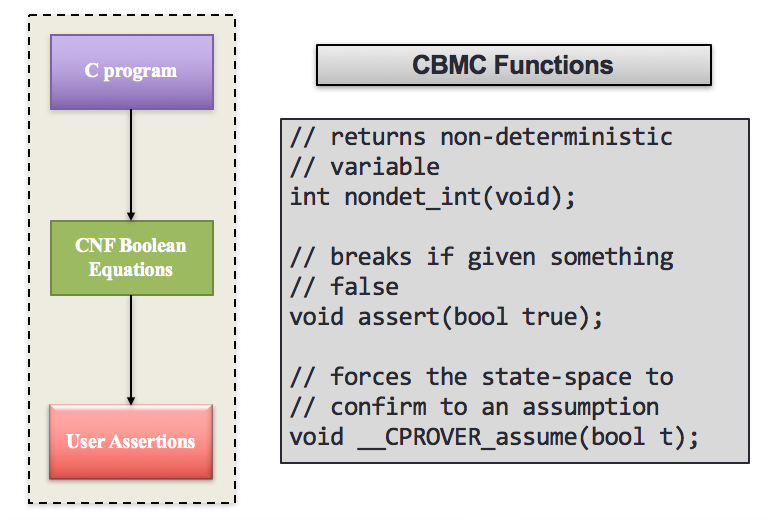
\includegraphics[width=0.8\linewidth]{CBMC_api.png}
  \caption{The figure on the left describes the transformation that a C
  program undergoes to be verified. The right describes the CBMC API.}\label{fig:CBMC_api}
\end{figure}

As we can see from Figure~\ref{fig:CBMC_api}, the CMBC API is very simple.
The \code{assert} function is the function used to describe the properties that
were outlined in the last section. 
The function takes in a boolean expression, and it is straightforward to
transform the propositional logic to a boolean expression in C.
If the boolean expression evaluates to \code{False}, then CBMC throws an error
and a ``counterexample''.
This counterexample is all of the program inputs and steps that led to this
assertion being False.
The \code{nondet\_int} function is used to model user input to the Vboot process.
Any data that could be modified by the user could feasibly take any
value.
To model this, \code{nondet\_int} is a function that returns a
``non-deterministic'' integer. 
Non-deterministic means the return integer can take any value, and CBMC
exhaustively checks user assertions against all possible integer values.

\subsubsection{Known CBMC Limitations}

In order to get CBMC running, certain limitations had to be observed.
The SAT generator of CBMC unrolls loops before converting the code into a model that can be checked.
This loop unroller is not able to unroll loops where the upperbound is data dependant, so these loops must either be avoided, or a limitation can be placed on the unrolling through the commandline. 
If the manually unrolling limitation is too small, then CBMC results may be incorrect, while if the limit is too large the state space may be too large for CMBC to finish in a reasonable time.
% TODO: may want to remove this bit about Memcpy
Luckily there was only a single loop of this nature, which existed in the method "Memcpy".
Using the C implementation of Vboot I was able to determine that Memcpy needed no more than 1050 loop unrollings for the data driven portion of Vboot.

\subsection{Verifying Vboot with CBMC}

CBMC was able to be successfully run on portions of the verified boot library and provide information on the satisfiability of various assertions.
Running CBMC on the Read-Only section of Vboot with a full Firmware Image is not possible as the program will consume up to 4GB of RAM on my local machine and then be cancelled.
In order to check properties, abstractions needed to be found such that parts of the Vboot flow could be checked at a single time.
The key insight that was used for this project is that individual functions are essentially self contained and can be abstracted away based on the properties that one desires to check.
Each function throughout Vboot returns an error code if it is not successful.
When a function is abstracted away, it is programmed to return a
non-deterministic value.
If the non-deterministic value is zero (success), then the minimal amount of external changes (if any) should be applied to the larger function.
If the abstracted function returns non-zero (error), then the external changes should be replaced with non-deterministic values.

This method is an over-abstraction of a functions found in the Vboot library.
An over-abstraction contains the full set of states found in the original function, plus additional states that would not be possible.
Because the over-abstraction is a super-set of the original states, any properties that are proved with the over-abstraction will also be proved on every state of the original function.
Therefore any properties proved with abstracted functions will also hold if the real functions were left in place.

\begin{figure}
  \centering
  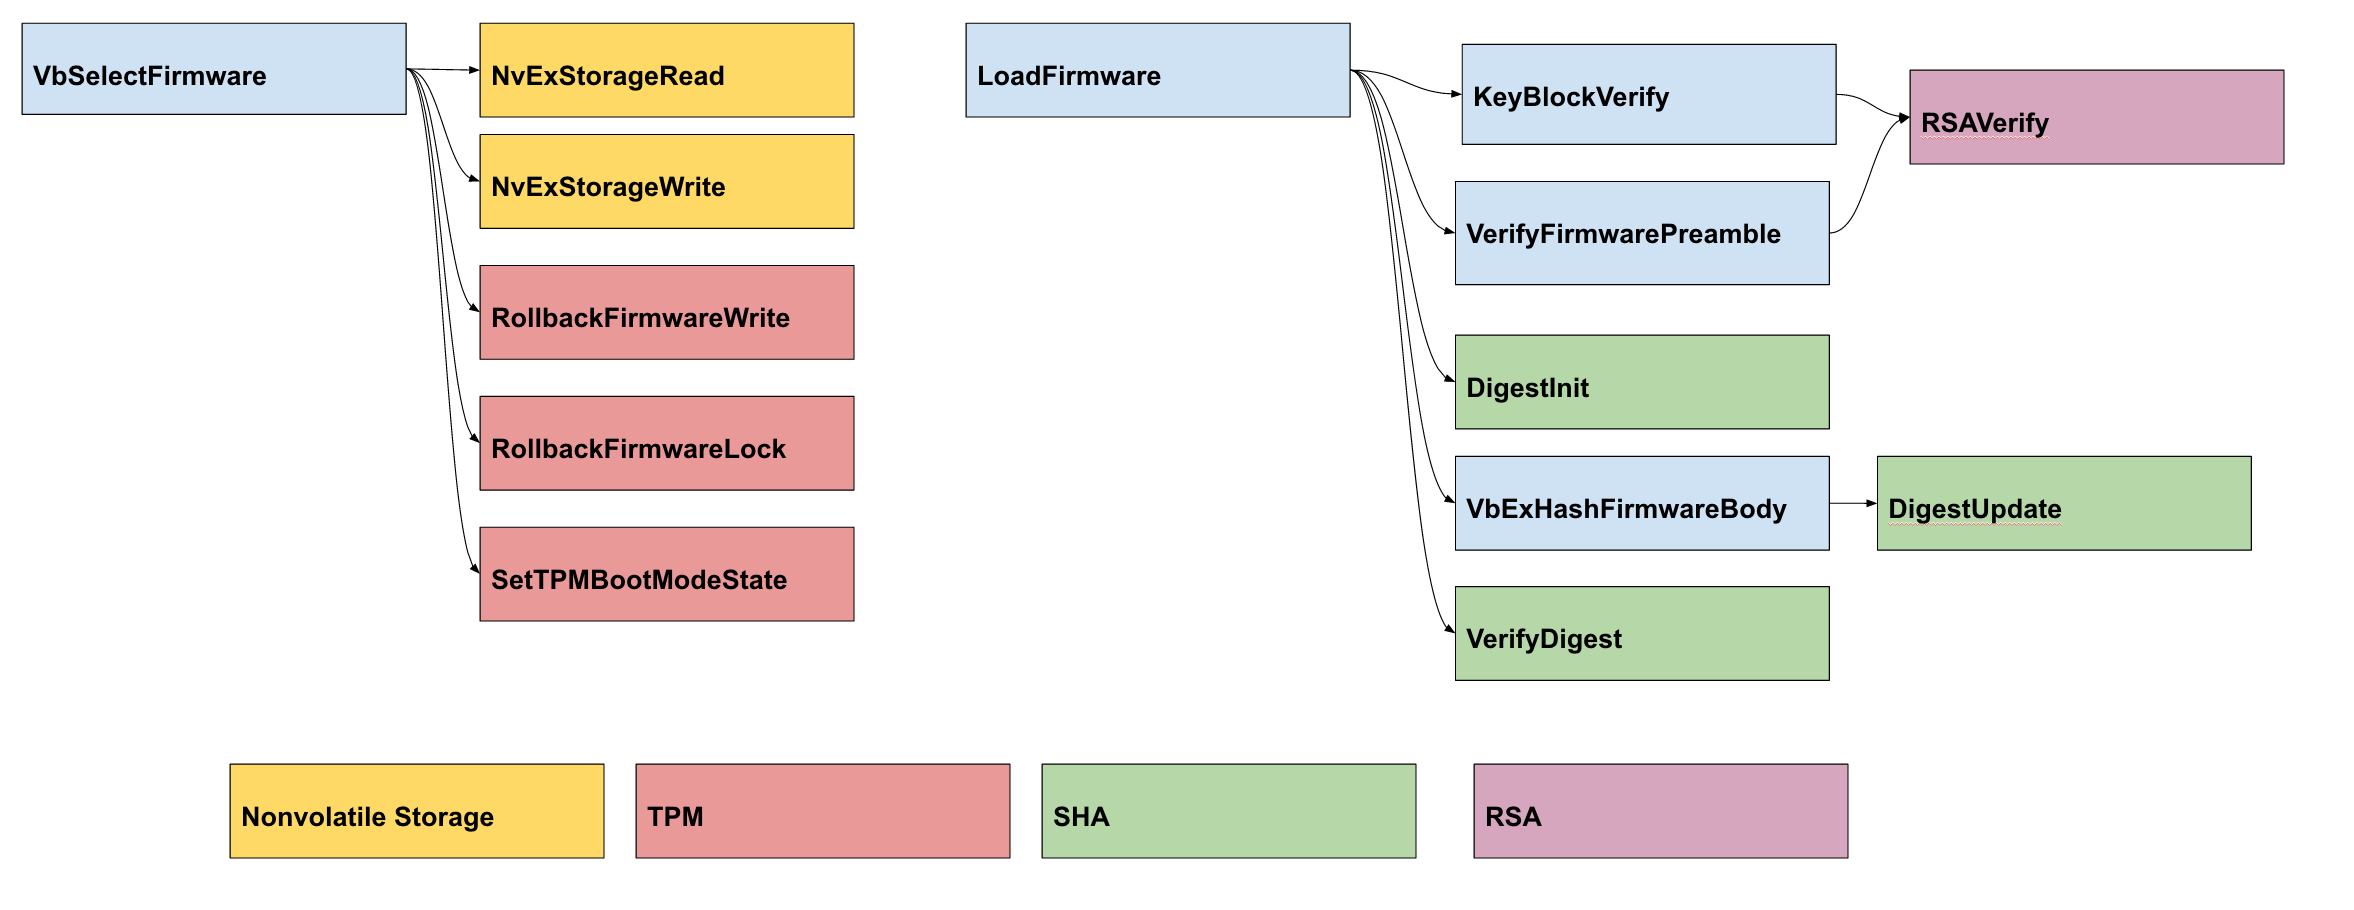
\includegraphics[width=0.8\linewidth]{ro_full_functions.png}
  \caption{The call graph of functions for Read Only Firmware}\label{fig:full_functions}
\end{figure}

The full graph of functions can be seen in Figure~\ref{fig:full_functions}.
The blue functions are fully software functions that are implemented in the Vboot Library.
The yellow functions connect to the Flash firmware on a real platform, but have been abstracted to return either non-deterministic data for Read-Write information, or hardcoded data for Read-Only information.
The red functions connect to the TPM on a real platform, but have been abstracted to return static variables are non-deterministic at the program's start.
The purple functions connect to either an RSA accelerator or a software RSA library. Instead of going through the full RSA algorithm, the function has been abstracted to a simple non-deterministic return of true or false. 
The green functions connect to either an SHA accelerator or a software SHA library.
The SHA algorithm has been abstracted in the same manner as RSA to return simply true or false at random.

For each of the next sections I will explain the verification process for individual functions. 
This explanation will include the function abstractions that were necessary, and a description of each of the tests run. 
There will be a table describing the results of each run of CBMC\@.
CMBC uses an implementation of a SAT solver known as the MiniSat solver\cite{minisat}.
This solver outputs unSAT if the assertions hold and SAT if they do not. 

\subsubsection{LoadFirmware}

The LoadFirmware function is where the main work is done in the Read-Only Vboot process.
LoadFirmware is responsible for calling functions that  Keyblock, Preamble, and Image verification.
When LoadFirmware returns, it will have set the pass or fail statuses of both Firmware Images.

All CBMC test results can be seen in Table~\ref{ldfw_results}. 
The Google unit tests involve adding a wrapper around Google's assertions within Vboot such that they hook into CBMC assertions.
This test shows that CMBC can be easily adapted into an existing framework and prove that Google specific assertions will not be thrown under any input.
The Rollback test checks that under no input conditions will LoadFirmware choose a firmware image with a lower version number (see Property~\ref{eq:rollback}).
In order to check that Rollback was working correctly, Rollback/rec tests that for rollback conditions without realizing that Rollback is allowed under recovery. 
The Rollback/Dev test correctly finds the counter-example where rollback is allowed and we can see that the recovery flag is enabled.
Hash Failure tests Property~\ref{eq:hash_cor}, or that it is impossible to verify an image as correct if the VbExHashFirmwareBody function returns an error.
RSA Failure tests Property~\ref{eq:sig_cor}, or that is impossible to verify an image as correct if the RSA key is formatted incorrectly or one of the Verify functions returns an error.
Array accesses check for all array bounds errors.

\begin{table}[]
    \centering
    \caption{CBMC tests on the LoadFirmware function}\label{ldfw_results}
    \begin{tabular}{|l|l|l|l|l|l|l|l|}
        \hline
        test name & steps & VCCs & vars  & clauses & time (s) & sat/unsat  \\ \hline \hline
        Google unit\_tests & 6460 & 34 & 1095643 & 24391723 & 67.02 & unsat \\ \hline
        rollback     & 4125 & 1 & 135239 & 1026823 & 4.79 & unsat \\ \hline
        rollback/rec & 4123 & 1 & 135276 & 1026983 & 4.68 & sat \\ \hline
        Hash Failure & 4182 & 2 & 137431 & 1043724 & 4.45 & unsat \\ \hline
        RSA  Failure & 4180 & 2 & 137825 & 1043921 & 4.45 & unsat \\ \hline
        Array Accesses & 4130 & 22 & 102660 & 640715 & 4.51 & unsat \\ \hline
    \end{tabular}
\end{table}

We can see from these tests that CBMC is working successfully and in a reasonable time.
The Google unit test framework is can be put to use with the CBMC framework using minor modifications, and the formal verification can be done in a very reasonable time.

\subsubsection{VbSelectFirmware}

The VbSelectFirmware function is the wrapper around LoadFirmware.
It is responsible for loading flags in from secure storage and for accessing the TPM\@.
VbSelectFirmware is also responsible for locking the TPM's firmware version before control passes to the firmware image and updating the version if a newer image has been loaded.
This function's final responsibility is to load TPM's PCR0 with the hash of the boot flags.

The TPM test for for this function is a series of correction properties. 
These assertions claim that the TPM must always be locked, and that VbSelectFirmware will not be successful if any of the TPM functions return an error.

The LoadFirmware test for this function simply checks that VbSelectFirmware will not not be successful if LoadFirmware returns an error.
This is necessary for the properties checked in LoadFirmware to propagate up to the entire boot flow, and it is what allows for our function abstractions.

\begin{table}[]
    \centering
    \caption{CBMC tests on function VbSelectFirmware}\label{sfw_results}
    \begin{tabular}{|l|l|l|l|l|l|l|l|}
        \hline
        test name & steps & VCCs & vars  & clauses & time (s) & sat/unsat  \\ \hline \hline
        TPM locking & 6 & 5269 & 13513 & 16784 & 0.07 & unsat \\ \hline
        LoadFirmware & 2 & 5264 & 13404 & 16209 & 0.07 & unsat \\ \hline
        Array Accesses & 5257 & 0 & 0 & 0 & 0 &  unsat \\ \hline
    \end{tabular}
\end{table}

\subsection{TPM Properties}

The Read-Only Firmware is responsible for setting up the TPM and protecting its
sections against the rest of the system that will eventually be loaded.
TPM's responsibilities from Chrome are to securely store the boot state and to protect against rollback attacks. 
Chrome's responsibilities for the TPM are to make sure that it is lead through
its self-check, that physical presence is disabled, and that the data zones
required by Chrome exist within the TPM's non-volatile state.

% Physical Presence
% http://www.trustedcomputinggroup.org/wp-content/uploads/Physical-Presence-Interface_1-30_0-52.pdf pg 19
Chrome disables the physical protection in the RO Firmware.
Physical presence is something that can be set high or low on a TPM either through software commands or a hardware wire. 
If Physical Presence is set high, then the ownership of the TPM can be changed and the re-provisioning operations become available.
For this reason, Chrome completely disables this option by permanently locking the TPM to a low Physical Presence\@.

% Rollback Attack
% TODO: Rollback attack visual
The other thing that the TPM protects from is Rollback Attacks.
In this situation a rollback attack is when older software with known
vulnerabilities replaces newer, protected software in a malicious ``upgrade.''
This attack works against a naive implementation because the attacker is relying on an older version of ChromeOS that is available, and unmodified.
Because the attacker is using Google's software, the software is signed by Google's private key and will be accepted by the VBoot algorithm.

\subsubsection{ILA for Hardware}   

\subsubsection{Verifying TPM with ILA}   
\clearpage

\end{document}

\documentclass[../report.tex]{subfiles}
\def\code#1{\texttt{#1}}
\begin{document}

\onehalfspacing
\newpage

\section{Security Recommendations}

This section will combine the results in the last section to provide security
recommendations for Verified Boot.
While no security holes were found in Verified Boot, specific additions to the
Vboot process would reduce the surface of attack in the future.
Reducing the surface of attack would also allow other properties to be proven
which would be more desirable.

\subsection{Memory Locking}

The biggest improvement to Verified Boot would be the addition of Memory
Locking.
Other Secure Boot implementations add hardware which enables locking sections
of RAM\cite{elane}.
This feature would help prove the security of Verified Boot by isolating it from
any external repositories.

As mentioned in the Software chapter, Verified Boot makes function calls into
the Coreboot and Depthcharge repositories.
If the Firmware Image is not locked before these function calls are made, then
it is possible that the image is corrupted before the control returns back to
Verified Boot.
The Coreboot and Depthcharge repositories together contain 415,035 lines. 
Compare this to the 16,000 lines in the Vboot repository and it is unlikely that
Formal Verification could check that the other repositories do not corrupt the
Image.

%TODO: Add locking image

The flow in Image~\ref{} shows an example of how the hardware locking would be
implemented.
This would prevent any Time of Check Time of Use (TOCTOU) Vulnerabilities that
would exist outside of the Verified Boot library.
% TODO: Add another reference here
TOCTOU vulnerabilities are very common in secure programs\cite{tpm-toctou}.

This recommendation was brought to the attention of Google Engineer's through
the Chromium-OS email group.
Their response was that it is possible to implement under current hardware, and
it was recommended under NIST's ``Bios Protection Guidelines'', but it has not
been implemented yet.

Implementing this feature would allow a formal proof that the Image is not
altered after being verified but before being executed. 
Until this feature is implemented, there will always be the possibility of a
TOCTOU attack vector.

\subsection{TPM Key Storage}

% TODO: Do the hashing and encrypting on the TPM
% This would actually help because people could fake the hash

\end{document}

\documentclass[../report.tex]{subfiles}
\begin{document}
\onehalfspacing

\section{Conclusion}

Throughout this paper, we investigated the importance and feasibility of formally verifying a large scale system.
Google's Verified Boot program was shown to be a good candidate for formal verification because of its security guarantees and its interactions across the hardware firmware boundary.
Verified Boot's properties were expressed formally using CTL and many were verified against the C implementation using the model checker CMBC\@. 
Model checking abstractions were discussed, such as abstracted functions, memory
allocation, and non-deterministic array writes.
These abstractions were necessary for Formal Verification tools to produce
results on the Verified Boot software.
Additionally, model checking was shown to be a good replacement for the unit
testing assertions which is already in place throughout Verified Boot.

\subsection{Future Work}

The analysis on Verified Boot is helpful in the way that it can be applied to
other systems. 
Verified Boot was chosen because it is a widely used code base
that crosses the Hardware Firmware boundary. 
Now that it has been shown that analysis can work on real systems, academic
work can be done on systems with more interesting behavior.
Verified Boot uses Hardware, but there are very little opportunities for
problems involving Hardware concurrency.
Other systems include interweaving uses of non-blocking
Hardware\cite{load-protocol} and these systems would showcase more strengths of the ILA functionality. 

One direction for the ILA toolchain that has been considered but not explored
is its use to verify that two hardware modules have the same functionality.
This direction is important as there are many TPM's produced by various Hardware
Vendors\cite{atmel-tpm}\cite{broadcom-tpm}\cite{infineon-tpm}, and the different 
implementations have been found to vary significantly\cite{tcg-inside}.
A full ILA description of a TPM would be very useful for comparing two hardware
chips from different vendors, as well as verifying that a software
implementation matches the Hardware implementation. 
Once the entire TPM functionality exists in an ILA description, more
verification could be done on the TPM API
itself\cite{TPM-state}\cite{TPM-spec-verif}.

Additionally, there are more areas in Google's Verified Boot that
deserve more attention. 
The Read-Write section of Verified Boot is ignored because it shares the
majority of its code with the Read-Only section, but it also contains a few
possibilities for attacks.
The Update functionality of Verified Boot should also be worth mentioning,
although this report already assumes that an attacker can upload arbitrary
updates.

In the future it is possible to extend the techniques in this paper to the rest of
Verified Boot or other exciting academic projects.




\end{document}

\appendix
\chapter{Code Organization}

The code for this report is based off of Google's Verified Boot reference repository\cite{vboot-codebase} and the modifications can be accessed in a cloned and edited repository\cite{my-repo}.
Changes were to the Verified Boot repo were mostly restricted to the main Makefile and the unit test folder \code{tests/}.

In order to have the results reproducible, all work was done inside of Vagrant Virtual Machine running Fedora 23. 
To get a working environment, clone the repository, initialize the Vagrant box, and run the following command:
\begin{equation}
    \code{\$PATH/CBMC-Vboot/scripts/install-fedora.sh} 
\end{equation}
This script will install the 49 packages required to run all of the code. 
Next, restart the Vagrant box and run the initialization script with:
\begin{equation}
    \code{\$PATH/CBMC-Vboot/scripts/init-fedora.sh} 
\end{equation}
This script will compile the 6 packages that need specific configurations.

The installation process takes roughly an hour on my 2015 Macbook Pro and the resulting VM image requires 4 Gbs of Hard Drive space. 

The \code{scripts/} folder contains the configuration scripts.
The main scripts are for installation, but there are also scripts to manage the SW TPM library, and to build a Vboot Image with related Public/Private keys.

The \code{qemu/} folder contains all of the code to run Vboot within QEMU with the hardware setup described in Section~\ref{qemu_em}.
The \code{tpm-pcr.c} file tests the only the TPM PCR functionality.
The \code{tpm-badcmds.c} file stress tests the TPM behavior with bad commands.
The \code{vboot-full.c} goes through the full process of Chrome's Verified Boot.
The \code{README.md} file contains information on building the software and using GDB testing.

The \code{CBMC/} folder contains all of the code for running Formal Verification on Vboot.
The python files with the naming structure \code{run\_\{\$FILE\}.py} will build and run the CBMC command for \code{\$FILE}.
The C files with the naming structure \code{test\_\{\$FILE\}.c} contain the main code being tested by CBMC\@.
The \code{README.md} file contains information on repeating the tests outlined in this report.


\section{CBMC Command Builder}
The code below shows the python script that builds a CBMC command for Formal Verification.
\lstinputlisting[language=Python]{code/cbmc.py}

\section{TPM Firmware}
This code shows the TPM read and write functionality.
\lstinputlisting[language=C]{code/tpm.c}

\section{TPM ILA}
This code shows the ILA for the TPM Hardware
\lstinputlisting[language=Python]{code/TPM_ILA.py}

\chapter{Images and Charts} 

\section{Images}

\begin{figure}[!htbp]
  \centering
  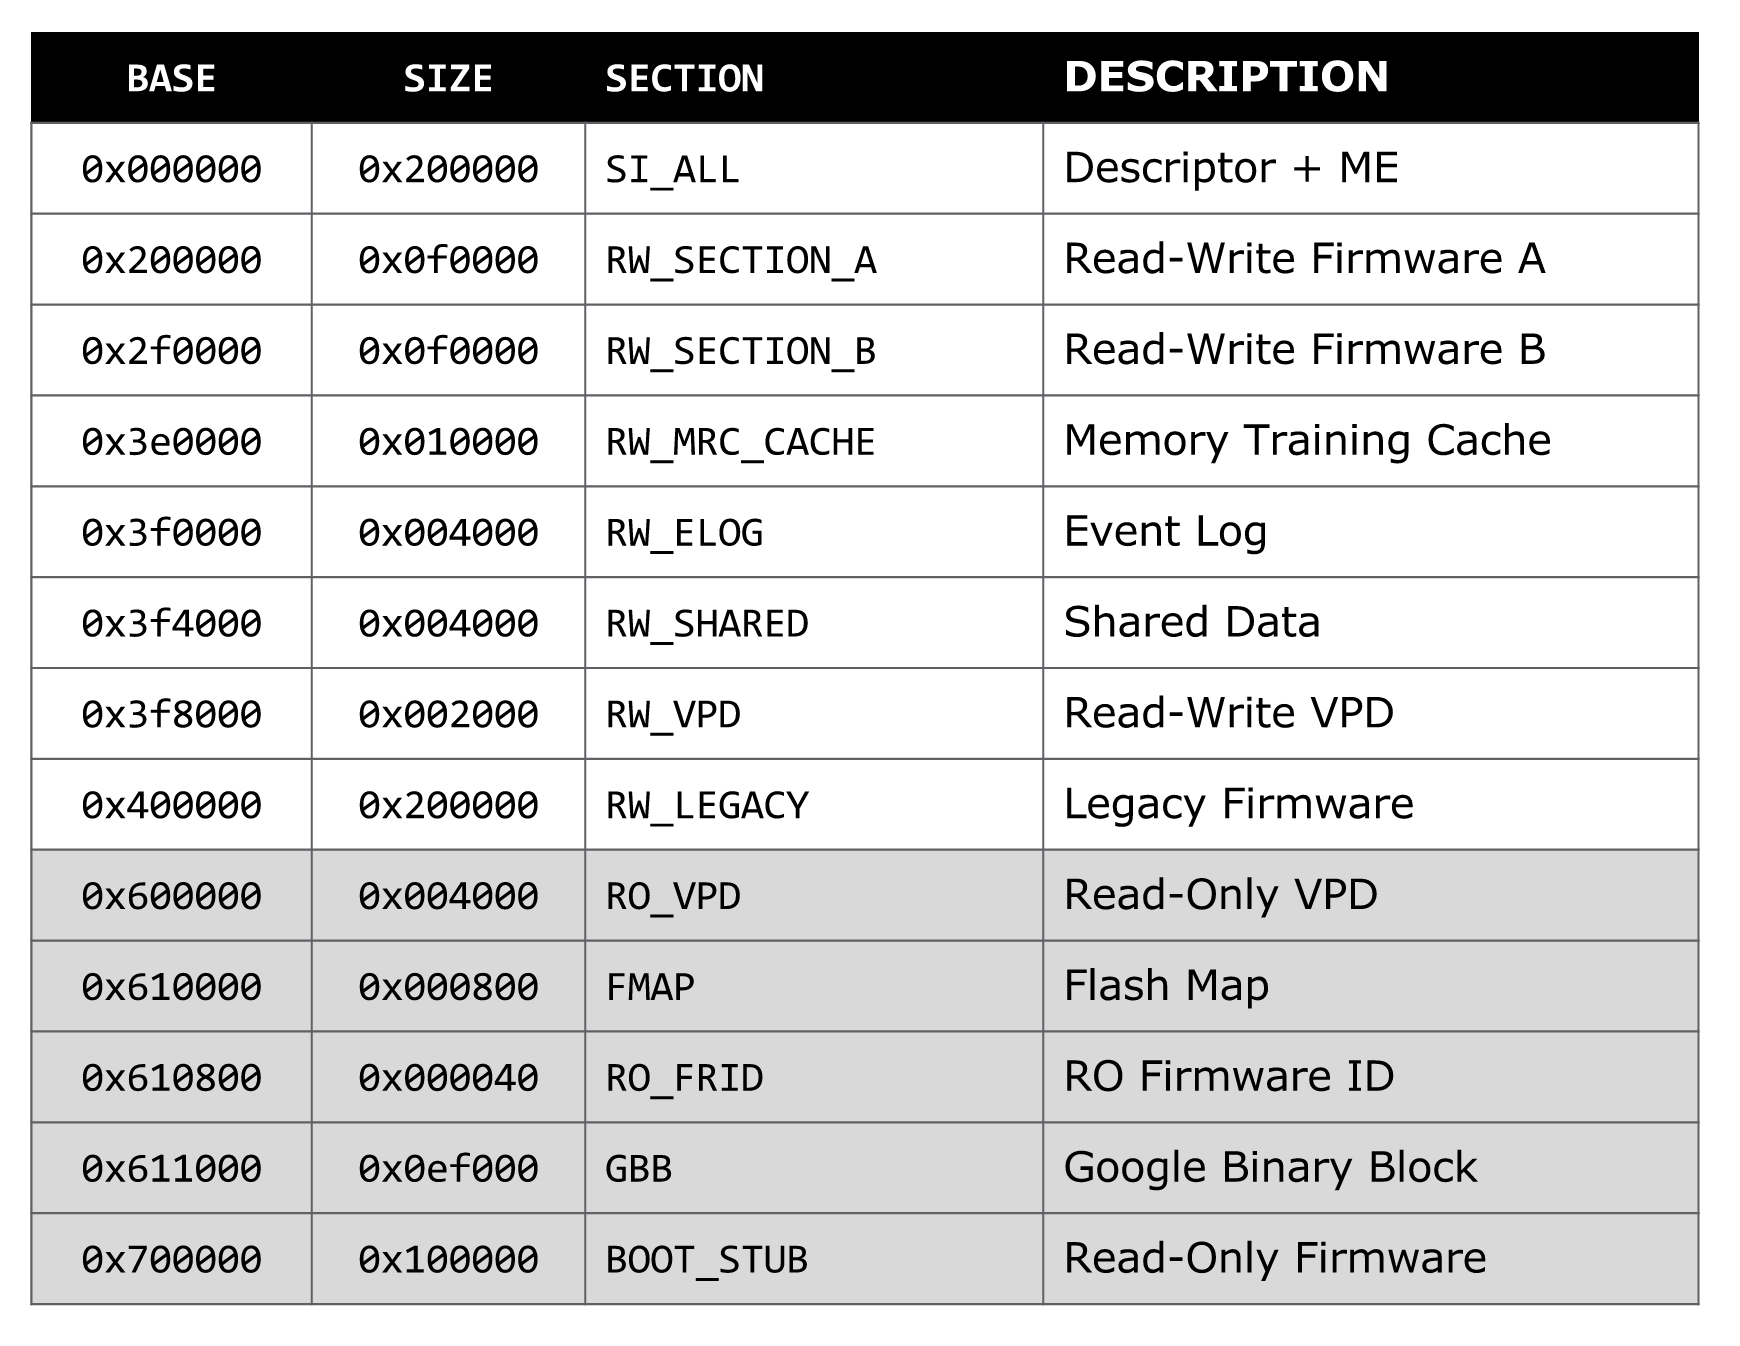
\includegraphics[width=0.8\linewidth]{fmap_locs.png}
  \caption[Chrome OS's Flash Map]{The Flash Map for Chrome OS's SPI Flash. The gray sections have been marked as Read Only~\cite{fw-summit}}
  \label{fig:fmap}
\end{figure}

\begin{figure}[!htbp]
  \centering
  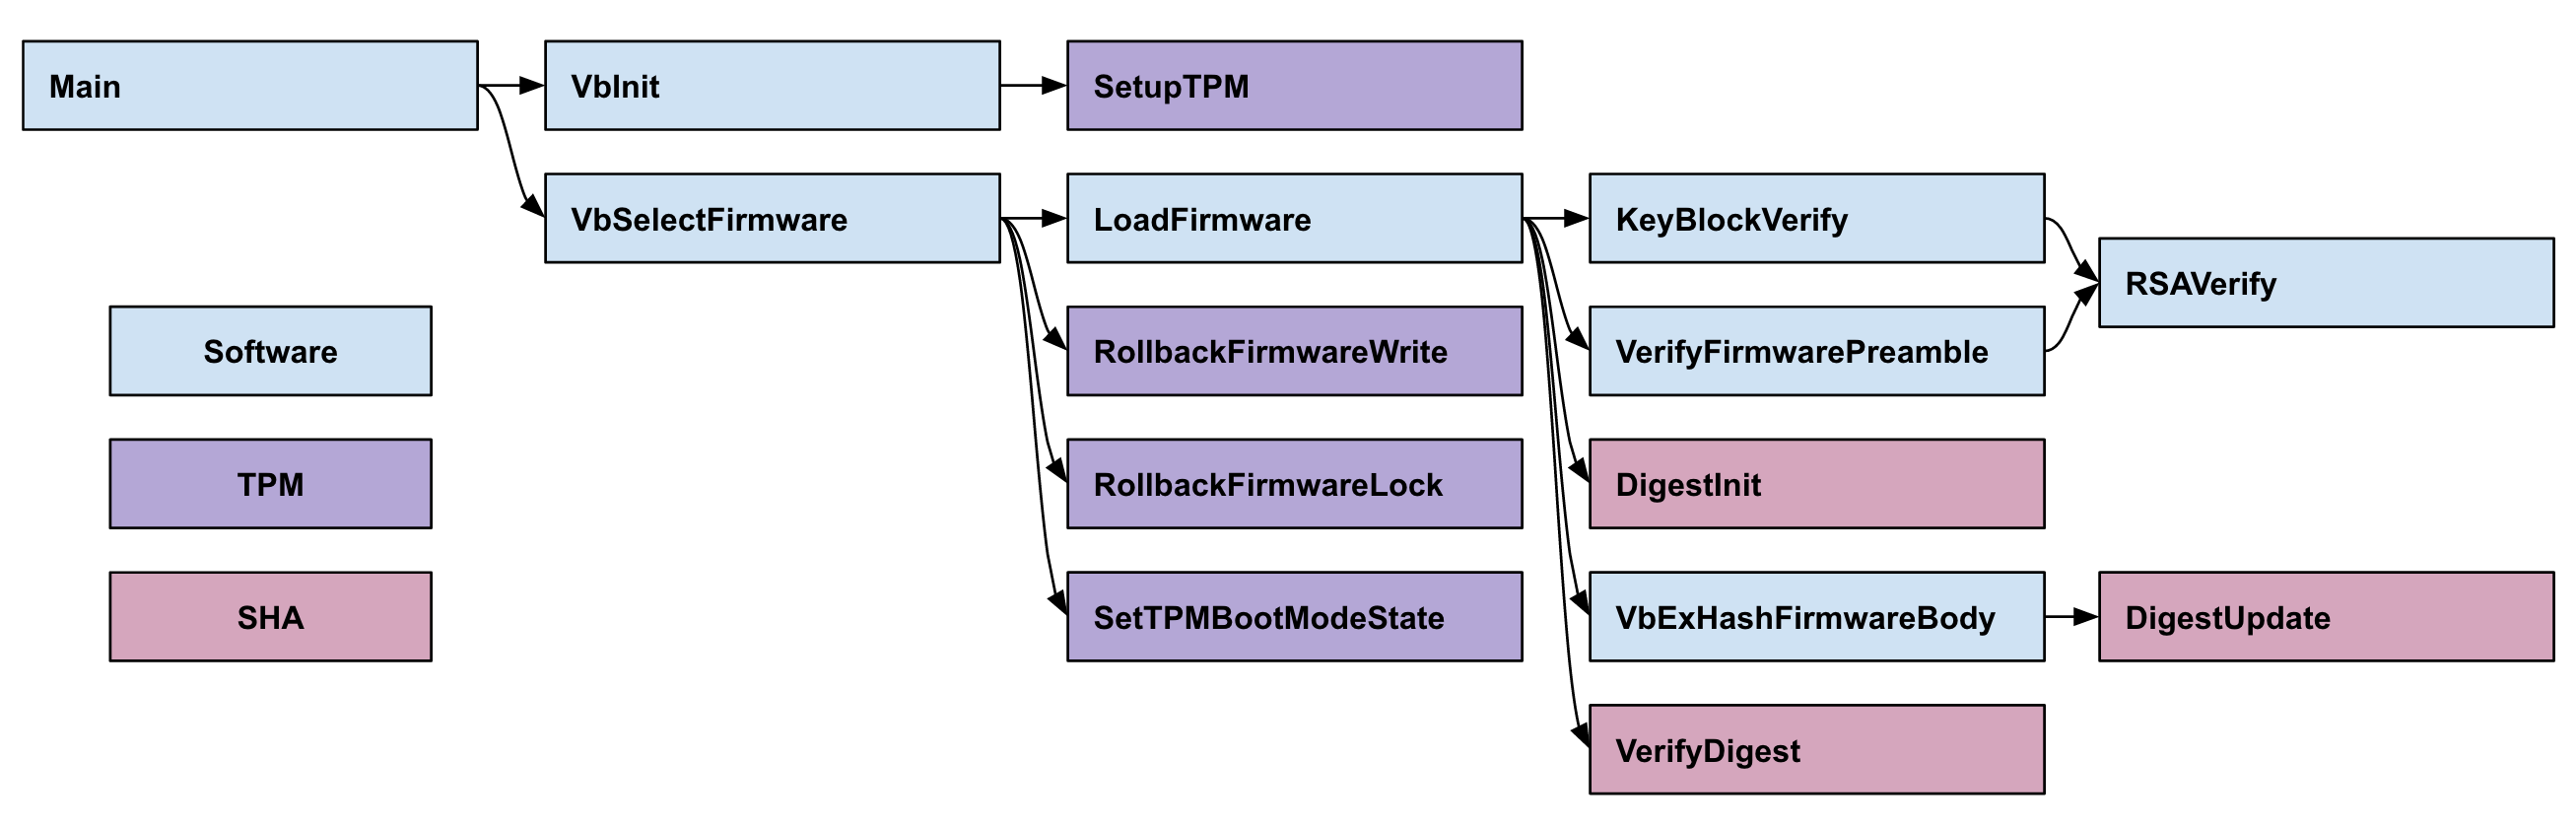
\includegraphics[width=1\linewidth]{full_flow.png}
  \caption{The full function call graph for Verified Boot}
  \label{fig:full_flow}
\end{figure}

\clearpage
\pagebreak

\begin{table}[!htbp]
    \centering
    \caption{All CBMC Tests}\label{all_results}
    \begin{tabular}{lrrrrr}
        \toprule
        test name & steps & VCCs & time (s) & memory (Mb) & sat/unsat  \\ \bottomrule
        Google Assertions & 6460 & 34 & 123 & 2312 & sat \\
        rollback     & 4125 & 1 & 4 & 259 & unsat \\
        rollback/rec & 4123 & 1 & 6 & 394 & sat \\
        Hash Failure & 4182 & 2 & 5 & 258 & unsat \\
        RSA  Failure & 4180 & 2 & 5 & 258 & unsat \\
        Array Accesses & 4130 & 57 & 126 & 2487 & unsat \\\midrule
        Google Assertions & 6460 & 34 & 3799 & 60496 & unsat \\
        Rollback, Hash, RSA & 2858 & 6 & 3733 & 59874 & unsat \\\midrule
        TPM locking & 5269 & 6 & 2 & 164 & unsat \\
        LoadFirmware & 5264 & 2 & 3 & 164 & unsat \\
        Array Accesses & 5257 & 10 & 3 & 165 &  unsat \\\midrule
        TPM Liveness & 20393 & 2220 & 387 & 15288 & unsat \\
        TPM Error Handling & 20109 & 3 & 379 & 15281 & unsat \\
        TPM Data Receive &  &  & & \\ \midrule
        TLCL Error Handling & & & & \\
        SetupTPM & 613418 & 140 & 1674 & 6960 & unsat \\
        RollbackFirmwareWrite & 478639 & 108 & 952 & 5447 & unsat \\
        RollbackFirmwareLock & 17450 & 4 & 7 & 369 & unsat \\
        SetTPMBootModeState & 34621 & 8 & 11 & 397 & unsat \\ \midrule
    \end{tabular}
\end{table}



% Make the bibliography single spaced
\singlespacing
\bibliographystyle{plain}

% add the Bibliography to the Table of Contents
\cleardoublepage
\ifdefined\phantomsection
  \phantomsection  % makes hyperref recognize this section properly for pdf link
\else
\fi
\addcontentsline{toc}{chapter}{Bibliography}

% include your .bib file
% \bibliography{thesis}
\begin{flushleft}
% Set font size
\begin{footnotesize}
% Actual Bibliography
\begin{thebibliography}{\kern\bibindent}

    \bibitem{greenstreet}
        C. Kern and M.R. Greenstreet, ``Formal verification in hardware design: a
        survey'', \textit{ACM Transactions on Design Automation of Electronic Systems (TODAES)}, v.4 n.2, p.123-193, April 1999 
    \bibitem{validating-sat}
        L. Zhang and S. Malik, ``Validating sat solvers using an independent resolution-based checker: Practical implementations and other applications,'' in \textit{Proceedings of the conference on Design, Automation and Test in Europe-Volume 1}, p. 10880, IEEE Computer Society, 2003.

    \bibitem{z3-smt-solver}
        L. De Moura and N. Bjørner, ``Z3: An Efficient SMT Solver'' in \textit{Internation conference on Tools and Algorithms for the Construction and Analysis of Systems.} Springer, Berlin. TACAS 2008. 

    \bibitem{hardware-accel}
        R. Weber et al., "Comparing Hardware Accelerators in Scientific Applications: A Case Study," in \textit{IEEE Transactions on Parallel and Distributed Systems}, vol. 22, no. 1, pp. 58-68, Jan. 2011.

    \bibitem{ila}
        S. Malik and S. Subramanyan, "Specification and Modeling for Systems-on-Chip Security Verification" Incomplete.

    \bibitem{ila-template}
        P. Subramanyan,  Y. Vizel, et-al "Template-based Synthesis of Instruction Level Abstractions for SoC Verification" Incomplete.

    \bibitem{elane}
E. Chou and S. Malik, "A Secure Bootloader for Demonstrating Formal Verification of Hardware-Firmware Interactions on SoCs" E.E. Princeton University, Princeton. NJ 2015

    \bibitem{security-basics}
        Lee, Ruby B. "Security basics for computer architects." Synthesis Lectures on Computer Architecture 8.4 (2013): 1-111.

    \bibitem{secure-bootloader}
        Cammack, William E., and Jason Douglas Kridner. "Secure bootloader for securing digital devices." U.S. Patent No. 7,237,121. 26 Jun. 2007.
    \bibitem{fw-summit}
        ``Chrome OS Firmware Overview'' Google Inc. Accessed Nov. 1, 2016. \url{https://docs.google.com/presentation/d/1h-nsDGlQmYI21dr95nYgLmyCYDgBIpJWSt9b7AqTZaw}        

    \bibitem{TPM}
        ``Trusted Platform Module'' Trusted Computing Group. Accessed Jan 10, 2016. \url{https://trustedcomputinggroup.org//work-groups/trusted-platform-module/}
    \bibitem{TCG}
        Trusted Computing Group. Accessed Jan. 10, 2016. \url{http://www.trustedcomputinggroup.org.}
    \bibitem{TPM-design}
        ``TPM Main: Part 1 Design Principles'' Trusted Computing Group.\url{https://trustedcomputinggroup.org/wp-content/uploads/Main-Part1-Rev94.pdf} Accessed Feb. 2 2017
    \bibitem{TPM-struct}
        ``TPM Main: Part 2 TPM Structures'' Trusted Computing Group.\url{https://trustedcomputinggroup.org/wp-content/uploads/TPM-main-1.2-Rev94-part-2.pdf} Accessed Feb. 2 2017
    \bibitem{TPM-cmd}
        ``TPM Main: Part 3 Commands'' Trusted Computing Group.\url{https://trustedcomputinggroup.org/wp-content/uploads/TPM-main-1.2-Rev94-part-3.pdf} Accessed Feb. 2 2017
    \bibitem{git}
        ``Git. Fast version Control'' Accessed Dec. 10, 2016. \url{https://git-scm.com/}
    \bibitem{vboot}
        ``Verified Boot'' Google Inc. Accessed Apr. 15, 2016. \url{https://www.chromium.org/chromium-os/chromiumos-design-docs/verified-boot}

    \bibitem{vboot-design-doc}
    ``Firmware Boot and Recovery'' Google Inc. Accessed Nov. 1, 2016. \url{http://www.chromium.org/chromium-os/chromiumos-design-docs/firmware-boot-and-recovery}

\bibitem{repo}
    ``Developing with Git and Repo'' Google Inc. Accessed Jan. 2, 2017. \url{http://source.android.com/source/developing.html}

\bibitem{coreboot}
    ``Coreboot'' Google Inc. Accessed Nov. 3, 2016. \url{https://www.coreboot.org/}

\bibitem{my-repo}
    ``CBMC-Vboot'' David Gilhooley. Accessed Mar. 6, 2017. \url{https://github.com/gilhooleyd/CBMC-Vboot}

\bibitem{coreboot-payload}
    ``Acquiring, Building, and Configuring the Payload Compatible with the Coreboot Reference Bootloader'' Intel. Dec 2015 \url{http://www.intel.com/content/dam/www/public/us/en/documents/white-papers/coreboot-reference-bootloader-white-paper.pdf}

\bibitem{depthcharge-slides}
    ``Depthcharge: The ChromeOS bootloader'' Google Inc. Accessed Nov. 3, 2016.
    \url{https://a77db9aa-a-7b23c8ea-s-sites.googlegroups.com/a/chromium.org/dev/chromium-os/2014-firmware-summit/ChromeOS\%20firmware\%20summit\%20-\%20Depthcharge.pdf}

\bibitem{depthcharge-codebase}
    ``Depthcharge Codebase'' Google Inc. Accessed Nov. 3 2016.\url{https://chromium.googlesource.com/chromiumos/platform/depthcharge/}

\bibitem{vboot-codebase}
    ``Verified Boot CodeBase'' Google Inc. Accessed Oct. 1 2016 \url{https://chromium.googlesource.com/chromiumos/platform/vboot\_reference/}

\bibitem{developer-mode}
    ``Chrome OS Developer Mode'' Google Inc. Accessed Nov 3 2016. \url{http://www.chromium.org/chromium-os/chromiumos-design-docs/developer-mode}

\bibitem{vboot-data-structures}
    ``Verified Boot Data Structures'' Google Inc. Accessed Nov 3 2016. \url{http://www.chromium.org/chromium-os/chromiumos-design-docs/verified-boot-data-structures}

\bibitem{minisat}
    N. Sorensson and N. Een. "Minisat v1. 13-a sat solver with conflict-clause minimization." \textit{SAT} 2005 
% \bibitem{my-repo}
%     D. Gilhooley. \url{https://bitbucket.org/david\_gilhooley/personal-vboot}, 2017
\bibitem{tpm-book}
    D. Challener. \textit{A Practical Guide To Trusted Computing}. 1st ed. Upper Saddle River, NJ: IBM Press/Pearson plc, 2008. Print.
\bibitem{tpm-slides}
    Ng, Raymond. \textit{TPM Fundamentals}. Infineon, APTISS. 2008. Slides.
\bibitem{qemu-site}
    ``QEMU: the Fast processor emulator'' \url{http://www.qemu-project.org/}
\bibitem{TPMLibs}
    Stefan, Berger. LibTpms. \url{https://github.com/stefanberger/libtpms} Accessed Feb 10 2017.
\bibitem{SWTPM}
    Stefan, Berger. SwTpm. \url{https://github.com/stefanberger/swtpm} Accessed Feb 10 2017.
\bibitem{TPMQEMU}
    Stefan, Berger. Qemu-Tpm. \url{https://github.com/stefanberger/qemu-tpm} Accessed Feb 10 2017.
\bibitem{multiboot}
    ``Multiboot Specification'' \url{https://www.gnu.org/software/grub/manual/multiboot/multiboot.html} Accessed Jan 5 2017.  \bibitem{trustfound}
    G. Bai et al. ``Trustfound: Towards a formal foundation for model checking trusted computing platforms.'' \textit{International Symposium on Formal Methods.} Springer International Publishing, 2014.
\bibitem{load-protocol}
    S. Krstic et al. ``Security of SoC firmware load protocols.''
    \textit{Hardware-Oriented Security and Trust (HOST), 2014 IEEE International Symposium on.} IEEE, 2014.
\bibitem{eff-model-check}
    F. Ivancic et al. ``Efficient SAT-based bounded model checking for software verification.'' \textit{Theoretical Computer Science 404.3} (2008): 256-274.
\bibitem{tpm-toctou}
    S. Bratus et al. ``TOCTOU, traps, and trusted computing.'' \textit{International Conference on Trusted Computing.} Springer Berlin Heidelberg, 2008.
\bibitem{bios-guidelines}
    D. Cooper et al. (2011). ``Bios protection guidelines''. \textit{NIST Special Publication, 800,} 147.
\bibitem{atmel-tpm}
     ``AT97SC3201 — The Atmel Trusted Platform Modul''. Atmel \url{http://www.atmel.com/images/doc5128.pdf} Accessed Apr 10 2017.
\bibitem{broadcom-tpm}
``BCM5752 -- Single-chip device for desktop lan-on-motherboard applications''. Broadcom. \url{http://www.recomb-omsk.ru/published/SC/html/scripts/doc/BCM5752-PB02-R.pdf} Accessed Apr 10 2017
\bibitem{infineon-tpm}
     ``Technologies AG. Product Brief — TPM 1.2 Hardware.'' Infineon. \url{http://www.infineon.com/tpm}, May 2005. Accessed Apr 10 2017
\bibitem{tcg-inside}
    A. Sadeghi et al. ``TCG inside?: a note on TPM specification compliance.'' \textit{Proceedings of the first ACM workshop on Scalable trusted computing.} ACM, 2006.
\bibitem{TPM-state}
    S. Delaune et al. ``A formal analysis of authentication in the TPM.'' in \textit{International Workshop on Formal Aspects in Security and Trust}. Springer Berlin Heidelberg, 2010.
\bibitem{TPM-spec-verif}
    S. Gurgens et al. ``Security evaluation of scenarios based on the TCG’s TPM specification.'' in \textit{European Symposium on Research in Computer Security}. Springer Berlin Heidelberg, 2007.
\bibitem{RoT}
    A. Regenscheid. "Roots of Trust in Mobile Devices", NIST, 2012. \url{http://csrc.nist.gov/groups/SMA/ispab/documents/minutes/2012-02/feb1\_mobility-roots-of-trust\_regenscheid.pdf} Accessed Apr 16 2017
\end{thebibliography}
\end{footnotesize}
\end{flushleft}

\end{document}

